% Options for packages loaded elsewhere
\PassOptionsToPackage{unicode}{hyperref}
\PassOptionsToPackage{hyphens}{url}
\PassOptionsToPackage{dvipsnames,svgnames,x11names}{xcolor}
%
\documentclass[
  letterpaper,
  DIV=11,
  numbers=noendperiod]{scrreprt}

\usepackage{amsmath,amssymb}
\usepackage{iftex}
\ifPDFTeX
  \usepackage[T1]{fontenc}
  \usepackage[utf8]{inputenc}
  \usepackage{textcomp} % provide euro and other symbols
\else % if luatex or xetex
  \usepackage{unicode-math}
  \defaultfontfeatures{Scale=MatchLowercase}
  \defaultfontfeatures[\rmfamily]{Ligatures=TeX,Scale=1}
\fi
\usepackage{lmodern}
\ifPDFTeX\else  
    % xetex/luatex font selection
\fi
% Use upquote if available, for straight quotes in verbatim environments
\IfFileExists{upquote.sty}{\usepackage{upquote}}{}
\IfFileExists{microtype.sty}{% use microtype if available
  \usepackage[]{microtype}
  \UseMicrotypeSet[protrusion]{basicmath} % disable protrusion for tt fonts
}{}
\makeatletter
\@ifundefined{KOMAClassName}{% if non-KOMA class
  \IfFileExists{parskip.sty}{%
    \usepackage{parskip}
  }{% else
    \setlength{\parindent}{0pt}
    \setlength{\parskip}{6pt plus 2pt minus 1pt}}
}{% if KOMA class
  \KOMAoptions{parskip=half}}
\makeatother
\usepackage{xcolor}
\setlength{\emergencystretch}{3em} % prevent overfull lines
\setcounter{secnumdepth}{5}
% Make \paragraph and \subparagraph free-standing
\ifx\paragraph\undefined\else
  \let\oldparagraph\paragraph
  \renewcommand{\paragraph}[1]{\oldparagraph{#1}\mbox{}}
\fi
\ifx\subparagraph\undefined\else
  \let\oldsubparagraph\subparagraph
  \renewcommand{\subparagraph}[1]{\oldsubparagraph{#1}\mbox{}}
\fi

\usepackage{color}
\usepackage{fancyvrb}
\newcommand{\VerbBar}{|}
\newcommand{\VERB}{\Verb[commandchars=\\\{\}]}
\DefineVerbatimEnvironment{Highlighting}{Verbatim}{commandchars=\\\{\}}
% Add ',fontsize=\small' for more characters per line
\usepackage{framed}
\definecolor{shadecolor}{RGB}{241,243,245}
\newenvironment{Shaded}{\begin{snugshade}}{\end{snugshade}}
\newcommand{\AlertTok}[1]{\textcolor[rgb]{0.68,0.00,0.00}{#1}}
\newcommand{\AnnotationTok}[1]{\textcolor[rgb]{0.37,0.37,0.37}{#1}}
\newcommand{\AttributeTok}[1]{\textcolor[rgb]{0.40,0.45,0.13}{#1}}
\newcommand{\BaseNTok}[1]{\textcolor[rgb]{0.68,0.00,0.00}{#1}}
\newcommand{\BuiltInTok}[1]{\textcolor[rgb]{0.00,0.23,0.31}{#1}}
\newcommand{\CharTok}[1]{\textcolor[rgb]{0.13,0.47,0.30}{#1}}
\newcommand{\CommentTok}[1]{\textcolor[rgb]{0.37,0.37,0.37}{#1}}
\newcommand{\CommentVarTok}[1]{\textcolor[rgb]{0.37,0.37,0.37}{\textit{#1}}}
\newcommand{\ConstantTok}[1]{\textcolor[rgb]{0.56,0.35,0.01}{#1}}
\newcommand{\ControlFlowTok}[1]{\textcolor[rgb]{0.00,0.23,0.31}{#1}}
\newcommand{\DataTypeTok}[1]{\textcolor[rgb]{0.68,0.00,0.00}{#1}}
\newcommand{\DecValTok}[1]{\textcolor[rgb]{0.68,0.00,0.00}{#1}}
\newcommand{\DocumentationTok}[1]{\textcolor[rgb]{0.37,0.37,0.37}{\textit{#1}}}
\newcommand{\ErrorTok}[1]{\textcolor[rgb]{0.68,0.00,0.00}{#1}}
\newcommand{\ExtensionTok}[1]{\textcolor[rgb]{0.00,0.23,0.31}{#1}}
\newcommand{\FloatTok}[1]{\textcolor[rgb]{0.68,0.00,0.00}{#1}}
\newcommand{\FunctionTok}[1]{\textcolor[rgb]{0.28,0.35,0.67}{#1}}
\newcommand{\ImportTok}[1]{\textcolor[rgb]{0.00,0.46,0.62}{#1}}
\newcommand{\InformationTok}[1]{\textcolor[rgb]{0.37,0.37,0.37}{#1}}
\newcommand{\KeywordTok}[1]{\textcolor[rgb]{0.00,0.23,0.31}{#1}}
\newcommand{\NormalTok}[1]{\textcolor[rgb]{0.00,0.23,0.31}{#1}}
\newcommand{\OperatorTok}[1]{\textcolor[rgb]{0.37,0.37,0.37}{#1}}
\newcommand{\OtherTok}[1]{\textcolor[rgb]{0.00,0.23,0.31}{#1}}
\newcommand{\PreprocessorTok}[1]{\textcolor[rgb]{0.68,0.00,0.00}{#1}}
\newcommand{\RegionMarkerTok}[1]{\textcolor[rgb]{0.00,0.23,0.31}{#1}}
\newcommand{\SpecialCharTok}[1]{\textcolor[rgb]{0.37,0.37,0.37}{#1}}
\newcommand{\SpecialStringTok}[1]{\textcolor[rgb]{0.13,0.47,0.30}{#1}}
\newcommand{\StringTok}[1]{\textcolor[rgb]{0.13,0.47,0.30}{#1}}
\newcommand{\VariableTok}[1]{\textcolor[rgb]{0.07,0.07,0.07}{#1}}
\newcommand{\VerbatimStringTok}[1]{\textcolor[rgb]{0.13,0.47,0.30}{#1}}
\newcommand{\WarningTok}[1]{\textcolor[rgb]{0.37,0.37,0.37}{\textit{#1}}}

\providecommand{\tightlist}{%
  \setlength{\itemsep}{0pt}\setlength{\parskip}{0pt}}\usepackage{longtable,booktabs,array}
\usepackage{calc} % for calculating minipage widths
% Correct order of tables after \paragraph or \subparagraph
\usepackage{etoolbox}
\makeatletter
\patchcmd\longtable{\par}{\if@noskipsec\mbox{}\fi\par}{}{}
\makeatother
% Allow footnotes in longtable head/foot
\IfFileExists{footnotehyper.sty}{\usepackage{footnotehyper}}{\usepackage{footnote}}
\makesavenoteenv{longtable}
\usepackage{graphicx}
\makeatletter
\def\maxwidth{\ifdim\Gin@nat@width>\linewidth\linewidth\else\Gin@nat@width\fi}
\def\maxheight{\ifdim\Gin@nat@height>\textheight\textheight\else\Gin@nat@height\fi}
\makeatother
% Scale images if necessary, so that they will not overflow the page
% margins by default, and it is still possible to overwrite the defaults
% using explicit options in \includegraphics[width, height, ...]{}
\setkeys{Gin}{width=\maxwidth,height=\maxheight,keepaspectratio}
% Set default figure placement to htbp
\makeatletter
\def\fps@figure{htbp}
\makeatother

\usepackage{booktabs}
\usepackage{longtable}
\usepackage{array}
\usepackage{multirow}
\usepackage{wrapfig}
\usepackage{float}
\usepackage{colortbl}
\usepackage{pdflscape}
\usepackage{tabu}
\usepackage{threeparttable}
\usepackage{threeparttablex}
\usepackage[normalem]{ulem}
\usepackage{makecell}
\usepackage{xcolor}
\usepackage{svg}
\KOMAoption{captions}{tableheading}
\makeatletter
\makeatother
\makeatletter
\@ifpackageloaded{bookmark}{}{\usepackage{bookmark}}
\makeatother
\makeatletter
\@ifpackageloaded{caption}{}{\usepackage{caption}}
\AtBeginDocument{%
\ifdefined\contentsname
  \renewcommand*\contentsname{Table of contents}
\else
  \newcommand\contentsname{Table of contents}
\fi
\ifdefined\listfigurename
  \renewcommand*\listfigurename{List of Figures}
\else
  \newcommand\listfigurename{List of Figures}
\fi
\ifdefined\listtablename
  \renewcommand*\listtablename{List of Tables}
\else
  \newcommand\listtablename{List of Tables}
\fi
\ifdefined\figurename
  \renewcommand*\figurename{Figure}
\else
  \newcommand\figurename{Figure}
\fi
\ifdefined\tablename
  \renewcommand*\tablename{Table}
\else
  \newcommand\tablename{Table}
\fi
}
\@ifpackageloaded{float}{}{\usepackage{float}}
\floatstyle{ruled}
\@ifundefined{c@chapter}{\newfloat{codelisting}{h}{lop}}{\newfloat{codelisting}{h}{lop}[chapter]}
\floatname{codelisting}{Listing}
\newcommand*\listoflistings{\listof{codelisting}{List of Listings}}
\makeatother
\makeatletter
\@ifpackageloaded{caption}{}{\usepackage{caption}}
\@ifpackageloaded{subcaption}{}{\usepackage{subcaption}}
\makeatother
\makeatletter
\@ifpackageloaded{tcolorbox}{}{\usepackage[skins,breakable]{tcolorbox}}
\makeatother
\makeatletter
\@ifundefined{shadecolor}{\definecolor{shadecolor}{rgb}{.97, .97, .97}}
\makeatother
\makeatletter
\makeatother
\makeatletter
\ifdefined\Shaded\renewenvironment{Shaded}{\begin{tcolorbox}[borderline west={3pt}{0pt}{shadecolor}, breakable, boxrule=0pt, interior hidden, frame hidden, enhanced, sharp corners]}{\end{tcolorbox}}\fi
\makeatother
\makeatletter
\makeatother
\ifLuaTeX
  \usepackage{selnolig}  % disable illegal ligatures
\fi
\IfFileExists{bookmark.sty}{\usepackage{bookmark}}{\usepackage{hyperref}}
\IfFileExists{xurl.sty}{\usepackage{xurl}}{} % add URL line breaks if available
\urlstyle{same} % disable monospaced font for URLs
\hypersetup{
  pdftitle={MetaDAG experiment example},
  pdfauthor={Version beta 0.2},
  colorlinks=true,
  linkcolor={blue},
  filecolor={Maroon},
  citecolor={Blue},
  urlcolor={Blue},
  pdfcreator={LaTeX via pandoc}}

\title{MetaDAG experiment example}
\author{Version beta 0.2}
\date{Invalid Date}

\begin{document}
\maketitle
\renewcommand*\contentsname{Table of contents}
{
\hypersetup{linkcolor=}
\setcounter{tocdepth}{2}
\tableofcontents
}
\bookmarksetup{startatroot}

\hypertarget{metadag-eukaryotes-experiment}{%
\chapter*{MetaDag Eukaryotes
experiment}\label{metadag-eukaryotes-experiment}}
\addcontentsline{toc}{chapter}{MetaDag Eukaryotes experiment}

\markboth{MetaDag Eukaryotes experiment}{MetaDag Eukaryotes experiment}

This is an example of an experiment of
\href{https://http://bioinfo.uib.es/metadag/}{metaDag} data with
results.

Hash: ff15c187-62e7-37c2-96a7-c824f7eab671

URL:
\url{http://bioinfo.uib.es/metadag/results?uuid=ff15c187-62e7-37c2-96a7-c824f7eab671}

\begin{Shaded}
\begin{Highlighting}[]
\FunctionTok{library}\NormalTok{(tidyverse)}
\FunctionTok{library}\NormalTok{(igraph)}
\FunctionTok{library}\NormalTok{(ComplexHeatmap)}
\FunctionTok{library}\NormalTok{(viridis)}
\FunctionTok{library}\NormalTok{(circlize)}
\FunctionTok{library}\NormalTok{(plotly)}
\FunctionTok{library}\NormalTok{(randomcoloR)}
\FunctionTok{library}\NormalTok{(factoextra)}
\FunctionTok{library}\NormalTok{(RColorBrewer)}
\FunctionTok{library}\NormalTok{(kableExtra)}
\FunctionTok{library}\NormalTok{(igraph)}
\FunctionTok{library}\NormalTok{(GGally)}
\end{Highlighting}
\end{Shaded}

\includegraphics[width=0.3\textwidth,height=\textheight]{figures/screen_2.png}

\includegraphics[width=0.3\textwidth,height=\textheight]{figures/screen_3.png}

\includegraphics[width=0.3\textwidth,height=\textheight]{figures/screen_4.png}

\bookmarksetup{startatroot}

\hypertarget{load-data-metadag-experiment}{%
\chapter*{Load data MetaDag
experiment}\label{load-data-metadag-experiment}}
\addcontentsline{toc}{chapter}{Load data MetaDag experiment}

\markboth{Load data MetaDag experiment}{Load data MetaDag experiment}

\begin{Shaded}
\begin{Highlighting}[]
\NormalTok{experiment}\OtherTok{=}
  \StringTok{"results\_ff15c187{-}62e7{-}37c2{-}96a7{-}c824f7eab671"}
\NormalTok{path\_exp}\OtherTok{=}\FunctionTok{paste0}\NormalTok{(}\StringTok{"data/"}\NormalTok{,experiment,}\StringTok{"/data/"}\NormalTok{)}
\NormalTok{knitr}\SpecialCharTok{::}\FunctionTok{kable}\NormalTok{(}\FunctionTok{data.frame}\NormalTok{(}\AttributeTok{Directory\_files\_and\_folders=}\FunctionTok{dir}\NormalTok{(path\_exp),}
                        \AttributeTok{Type=}\FunctionTok{c}\NormalTok{(}\FunctionTok{rep}\NormalTok{(}\StringTok{"Data file"}\NormalTok{,}\DecValTok{2}\NormalTok{),}
                       \FunctionTok{rep}\NormalTok{(}\StringTok{"Directory"}\NormalTok{,}\DecValTok{2}\NormalTok{),}
                       \FunctionTok{rep}\NormalTok{(}\StringTok{"Data file"}\NormalTok{,}\DecValTok{6}\NormalTok{),}
                       \StringTok{"Directory"}\NormalTok{)))}
\end{Highlighting}
\end{Shaded}

\begin{tabular}{l|l}
\hline
Directory\_files\_and\_folders & Type\\
\hline
Different\_MBB.csv & Data file\\
\hline
Different\_mDAG.csv & Data file\\
\hline
Global & Directory\\
\hline
Individuals & Directory\\
\hline
Results.csv & Data file\\
\hline
Similarities\_MBB\_MSAMethod.csv & Data file\\
\hline
Similarities\_MBB\_MunkresMethod.csv & Data file\\
\hline
Similarities\_mDAG\_MSAMethod.csv & Data file\\
\hline
Similarities\_mDAG\_MunkresMethod.csv & Data file\\
\hline
Similarities\_mDAGOnReaction.csv & Data file\\
\hline
TaxonomyLevels & Directory\\
\hline
\end{tabular}

\begin{Shaded}
\begin{Highlighting}[]
\NormalTok{MBB}\OtherTok{=}\FunctionTok{read\_csv}\NormalTok{(}\FunctionTok{paste0}\NormalTok{(path\_exp,}\StringTok{"Different\_MBB.csv"}\NormalTok{),}\AttributeTok{show\_col\_types =} \ConstantTok{FALSE}\NormalTok{)}
\NormalTok{mDAG}\OtherTok{=}\FunctionTok{read\_csv}\NormalTok{(}\FunctionTok{paste0}\NormalTok{(path\_exp,}\StringTok{"Different\_mDAG.csv"}\NormalTok{),}\AttributeTok{show\_col\_types =} \ConstantTok{FALSE}\NormalTok{)}
\NormalTok{Results}\OtherTok{=}\FunctionTok{read\_csv}\NormalTok{(}\FunctionTok{paste0}\NormalTok{(path\_exp,}\StringTok{"Results.csv"}\NormalTok{),}\AttributeTok{show\_col\_types =} \ConstantTok{FALSE}\NormalTok{)}
\FunctionTok{save}\NormalTok{(MBB,mDAG,Results,}\AttributeTok{file=}\StringTok{"MBB\_mDag\_Results.Rdata"}\NormalTok{)}
\end{Highlighting}
\end{Shaded}

\hypertarget{mbb}{%
\section*{MBB}\label{mbb}}
\addcontentsline{toc}{section}{MBB}

\markright{MBB}

In this experiment \texttt{MBB} is a table with 5112 rows and 4106
columns.

\begin{Shaded}
\begin{Highlighting}[]
\NormalTok{knitr}\SpecialCharTok{::}\FunctionTok{kable}\NormalTok{(MBB[}\DecValTok{1}\SpecialCharTok{:}\DecValTok{20}\NormalTok{,}\DecValTok{1}\SpecialCharTok{:}\DecValTok{30}\NormalTok{]) }\SpecialCharTok{\%\textgreater{}\%}   \FunctionTok{scroll\_box}\NormalTok{(}\AttributeTok{width =} \StringTok{"100\%"}\NormalTok{, }\AttributeTok{height =} \StringTok{"200px"}\NormalTok{)}
\end{Highlighting}
\end{Shaded}

\begin{tabular}{l|r|r|r|r|r|r|r|r|r|r|r|r|r|r|r|r|r|r|r|r|r|r|r|r|r|r|r|r|r}
\hline
MBB Id & natural & \#pathways & Protists & Fungi & Plants & Animals & Alveolates & Amoebozoa & Annelids & Arthropods & Ascomycetes & Basal angiosperms & Basidiomycetes & Brachiopodas & Cephalochordates & Choanoflagellates & Cnidarians & Cryptomonads & Echinoderms & Eudicots & Euglenozoa & Ferns & Flatworms & Green algae & Haptophyta & Hemichordates & Heterolobosea & Metamonada & Microsporidians\\
\hline
0 & 0 & 0 & 0 & 0 & 0 & 0 & 0 & 0 & 0 & 0 & 0 & 0 & 0 & 0 & 0 & 0 & 0 & 0 & 0 & 0 & 0 & 0 & 0 & 0 & 0 & 0 & 0 & 0 & 0\\
\hline
0.0 & 0 & 0 & 0 & 0 & 0 & 0 & 0 & 0 & 0 & 0 & 0 & 0 & 0 & 0 & 0 & 0 & 0 & 0 & 0 & 0 & 0 & 0 & 0 & 0 & 0 & 0 & 0 & 0 & 0\\
\hline
0.0.0 & 1 & 1 & 1 & 0 & 0 & 0 & 0 & 0 & 0 & 0 & 0 & 0 & 0 & 0 & 0 & 0 & 0 & 0 & 0 & 0 & 0 & 0 & 0 & 0 & 0 & 0 & 0 & 0 & 0\\
\hline
0.0.0.0 & 1 & 1 & 1 & 0 & 0 & 0 & 0 & 0 & 0 & 0 & 0 & 0 & 0 & 0 & 0 & 0 & 0 & 0 & 0 & 0 & 0 & 0 & 0 & 0 & 0 & 0 & 0 & 0 & 0\\
\hline
0.0.1 & 1 & 1 & 1 & 0 & 0 & 0 & 0 & 0 & 0 & 0 & 0 & 0 & 0 & 0 & 0 & 0 & 0 & 0 & 0 & 0 & 0 & 0 & 0 & 0 & 0 & 0 & 0 & 0 & 0\\
\hline
0.0.1.0 & 1 & 86 & 2 & 77 & 1 & 6 & 1 & 0 & 0 & 5 & 57 & 0 & 20 & 0 & 0 & 0 & 0 & 0 & 0 & 0 & 0 & 0 & 0 & 0 & 1 & 0 & 0 & 0 & 0\\
\hline
0.0.1.1 & 1 & 86 & 2 & 77 & 1 & 6 & 1 & 0 & 0 & 5 & 57 & 0 & 20 & 0 & 0 & 0 & 0 & 0 & 0 & 0 & 0 & 0 & 0 & 0 & 1 & 0 & 0 & 0 & 0\\
\hline
0.0.1.2 & 1 & 15 & 15 & 0 & 0 & 0 & 12 & 0 & 0 & 0 & 0 & 0 & 0 & 0 & 0 & 0 & 0 & 0 & 0 & 0 & 0 & 0 & 0 & 0 & 0 & 0 & 0 & 0 & 0\\
\hline
0.0.1.3 & 1 & 5 & 5 & 0 & 0 & 0 & 0 & 4 & 0 & 0 & 0 & 0 & 0 & 0 & 0 & 0 & 0 & 0 & 0 & 0 & 0 & 0 & 0 & 0 & 0 & 0 & 1 & 0 & 0\\
\hline
0.0.1.4 & 0 & 0 & 0 & 0 & 0 & 0 & 0 & 0 & 0 & 0 & 0 & 0 & 0 & 0 & 0 & 0 & 0 & 0 & 0 & 0 & 0 & 0 & 0 & 0 & 0 & 0 & 0 & 0 & 0\\
\hline
0.0.1.4.0 & 1 & 609 & 14 & 128 & 128 & 339 & 1 & 3 & 1 & 8 & 93 & 2 & 35 & 1 & 2 & 2 & 4 & 0 & 3 & 98 & 0 & 1 & 3 & 3 & 1 & 1 & 1 & 1 & 0\\
\hline
0.0.1.4.1 & 1 & 609 & 14 & 128 & 128 & 339 & 1 & 3 & 1 & 8 & 93 & 2 & 35 & 1 & 2 & 2 & 4 & 0 & 3 & 98 & 0 & 1 & 3 & 3 & 1 & 1 & 1 & 1 & 0\\
\hline
0.0.1.4.2 & 1 & 322 & 6 & 92 & 133 & 91 & 1 & 0 & 0 & 61 & 62 & 2 & 30 & 1 & 2 & 1 & 8 & 0 & 2 & 98 & 0 & 1 & 0 & 7 & 1 & 1 & 1 & 0 & 0\\
\hline
0.0.1.4.3 & 1 & 322 & 6 & 92 & 133 & 91 & 1 & 0 & 0 & 61 & 62 & 2 & 30 & 1 & 2 & 1 & 8 & 0 & 2 & 98 & 0 & 1 & 0 & 7 & 1 & 1 & 1 & 0 & 0\\
\hline
0.0.1.4.4 & 1 & 1 & 0 & 0 & 1 & 0 & 0 & 0 & 0 & 0 & 0 & 0 & 0 & 0 & 0 & 0 & 0 & 0 & 0 & 0 & 0 & 0 & 0 & 0 & 0 & 0 & 0 & 0 & 0\\
\hline
0.0.1.4.5 & 1 & 1 & 1 & 0 & 0 & 0 & 0 & 1 & 0 & 0 & 0 & 0 & 0 & 0 & 0 & 0 & 0 & 0 & 0 & 0 & 0 & 0 & 0 & 0 & 0 & 0 & 0 & 0 & 0\\
\hline
0.0.1.5 & 0 & 0 & 0 & 0 & 0 & 0 & 0 & 0 & 0 & 0 & 0 & 0 & 0 & 0 & 0 & 0 & 0 & 0 & 0 & 0 & 0 & 0 & 0 & 0 & 0 & 0 & 0 & 0 & 0\\
\hline
0.0.1.5.0 & 1 & 5 & 5 & 0 & 0 & 0 & 0 & 4 & 0 & 0 & 0 & 0 & 0 & 0 & 0 & 0 & 0 & 0 & 0 & 0 & 0 & 0 & 0 & 0 & 0 & 0 & 1 & 0 & 0\\
\hline
0.0.2 & 1 & 1 & 1 & 0 & 0 & 0 & 0 & 0 & 0 & 0 & 0 & 0 & 0 & 0 & 0 & 0 & 0 & 0 & 0 & 0 & 0 & 0 & 0 & 0 & 0 & 0 & 0 & 0 & 0\\
\hline
0.0.3 & 1 & 1 & 1 & 0 & 0 & 0 & 0 & 1 & 0 & 0 & 0 & 0 & 0 & 0 & 0 & 0 & 0 & 0 & 0 & 0 & 0 & 0 & 0 & 0 & 0 & 0 & 0 & 0 & 0\\
\hline
\end{tabular}

\hypertarget{mdag}{%
\section*{mDAG}\label{mdag}}
\addcontentsline{toc}{section}{mDAG}

\markright{mDAG}

Abstract/unique mDAG's in this experiment

\begin{Shaded}
\begin{Highlighting}[]
\FunctionTok{dim}\NormalTok{(mDAG)}
\end{Highlighting}
\end{Shaded}

\begin{verbatim}
[1]  884 5224
\end{verbatim}

\begin{Shaded}
\begin{Highlighting}[]
\FunctionTok{kable}\NormalTok{(mDAG[}\DecValTok{1}\SpecialCharTok{:}\DecValTok{20}\NormalTok{,}\DecValTok{1}\SpecialCharTok{:}\DecValTok{30}\NormalTok{]) }\SpecialCharTok{\%\textgreater{}\%}   \FunctionTok{scroll\_box}\NormalTok{(}\AttributeTok{width =} \StringTok{"100\%"}\NormalTok{, }\AttributeTok{height =} \StringTok{"200px"}\NormalTok{)}
\end{Highlighting}
\end{Shaded}

\begin{tabular}{l|r|r|r|r|r|r|r|r|r|r|r|r|r|r|r|r|r|r|r|r|r|r|r|r|r|r|r|r|r}
\hline
mDAG Id & \#Categories & Animals & Plants & Fungi & Protists & Alveolates & Amoebozoa & Annelids & Arthropods & Ascomycetes & Basal angiosperms & Basidiomycetes & Brachiopodas & Cephalochordates & Choanoflagellates & Cnidarians & Cryptomonads & Echinoderms & Eudicots & Euglenozoa & Ferns & Flatworms & Green algae & Haptophyta & Hemichordates & Heterolobosea & Metamonada & Microsporidians & Mollusks\\
\hline
0001 & 3 & 1 & 0 & 0 & 0 & 0 & 0 & 0 & 0 & 0 & 0 & 0 & 0 & 0 & 0 & 0 & 0 & 0 & 0 & 0 & 0 & 0 & 0 & 0 & 0 & 0 & 0 & 0 & 0\\
\hline
0002 & 2 & 0 & 0 & 1 & 0 & 0 & 0 & 0 & 0 & 0 & 0 & 1 & 0 & 0 & 0 & 0 & 0 & 0 & 0 & 0 & 0 & 0 & 0 & 0 & 0 & 0 & 0 & 0 & 0\\
\hline
0003 & 2 & 1 & 0 & 0 & 0 & 0 & 0 & 0 & 0 & 0 & 0 & 0 & 0 & 0 & 0 & 0 & 0 & 0 & 0 & 0 & 0 & 1 & 0 & 0 & 0 & 0 & 0 & 0 & 0\\
\hline
0004 & 3 & 1 & 0 & 0 & 0 & 0 & 0 & 0 & 0 & 0 & 0 & 0 & 0 & 0 & 0 & 0 & 0 & 0 & 0 & 0 & 0 & 0 & 0 & 0 & 0 & 0 & 0 & 0 & 0\\
\hline
0005 & 3 & 1 & 0 & 0 & 0 & 0 & 0 & 0 & 0 & 0 & 0 & 0 & 0 & 0 & 0 & 0 & 0 & 0 & 0 & 0 & 0 & 0 & 0 & 0 & 0 & 0 & 0 & 0 & 0\\
\hline
0006 & 3 & 0 & 1 & 0 & 0 & 0 & 0 & 0 & 0 & 0 & 0 & 0 & 0 & 0 & 0 & 0 & 0 & 0 & 1 & 0 & 0 & 0 & 0 & 0 & 0 & 0 & 0 & 0 & 0\\
\hline
0007 & 2 & 0 & 1 & 0 & 0 & 0 & 0 & 0 & 0 & 0 & 0 & 0 & 0 & 0 & 0 & 0 & 0 & 0 & 0 & 0 & 0 & 0 & 0 & 0 & 0 & 0 & 0 & 0 & 0\\
\hline
0008 & 3 & 0 & 1 & 0 & 0 & 0 & 0 & 0 & 0 & 0 & 0 & 0 & 0 & 0 & 0 & 0 & 0 & 0 & 0 & 0 & 0 & 0 & 0 & 0 & 0 & 0 & 0 & 0 & 0\\
\hline
0009 & 3 & 0 & 1 & 0 & 0 & 0 & 0 & 0 & 0 & 0 & 0 & 0 & 0 & 0 & 0 & 0 & 0 & 0 & 1 & 0 & 0 & 0 & 0 & 0 & 0 & 0 & 0 & 0 & 0\\
\hline
0010 & 3 & 1 & 0 & 0 & 0 & 0 & 0 & 0 & 0 & 0 & 0 & 0 & 0 & 0 & 0 & 0 & 0 & 0 & 0 & 0 & 0 & 0 & 0 & 0 & 0 & 0 & 0 & 0 & 0\\
\hline
0011 & 3 & 1 & 0 & 0 & 0 & 0 & 0 & 0 & 0 & 0 & 0 & 0 & 0 & 0 & 0 & 0 & 0 & 0 & 0 & 0 & 0 & 0 & 0 & 0 & 0 & 0 & 0 & 0 & 0\\
\hline
0012 & 3 & 0 & 0 & 0 & 1 & 0 & 0 & 0 & 0 & 0 & 0 & 0 & 0 & 0 & 0 & 0 & 0 & 0 & 0 & 0 & 0 & 0 & 0 & 0 & 0 & 0 & 1 & 0 & 0\\
\hline
0013 & 3 & 1 & 0 & 0 & 0 & 0 & 0 & 0 & 0 & 0 & 0 & 0 & 0 & 0 & 0 & 0 & 0 & 0 & 0 & 0 & 0 & 0 & 0 & 0 & 0 & 0 & 0 & 0 & 0\\
\hline
0014 & 3 & 0 & 0 & 0 & 1 & 1 & 0 & 0 & 0 & 0 & 0 & 0 & 0 & 0 & 0 & 0 & 0 & 0 & 0 & 0 & 0 & 0 & 0 & 0 & 0 & 0 & 0 & 0 & 0\\
\hline
0015 & 2 & 0 & 0 & 1 & 0 & 0 & 0 & 0 & 0 & 0 & 0 & 0 & 0 & 0 & 0 & 0 & 0 & 0 & 0 & 0 & 0 & 0 & 0 & 0 & 0 & 0 & 0 & 1 & 0\\
\hline
0016 & 3 & 0 & 0 & 0 & 1 & 0 & 1 & 0 & 0 & 0 & 0 & 0 & 0 & 0 & 0 & 0 & 0 & 0 & 0 & 0 & 0 & 0 & 0 & 0 & 0 & 0 & 0 & 0 & 0\\
\hline
0017 & 3 & 1 & 0 & 0 & 0 & 0 & 0 & 0 & 0 & 0 & 0 & 0 & 0 & 0 & 0 & 0 & 0 & 0 & 0 & 0 & 0 & 0 & 0 & 0 & 0 & 0 & 0 & 0 & 0\\
\hline
0018 & 3 & 1 & 0 & 0 & 0 & 0 & 0 & 0 & 0 & 0 & 0 & 0 & 0 & 0 & 0 & 0 & 0 & 0 & 0 & 0 & 0 & 0 & 0 & 0 & 0 & 0 & 0 & 0 & 0\\
\hline
0019 & 3 & 1 & 0 & 0 & 0 & 0 & 0 & 0 & 1 & 0 & 0 & 0 & 0 & 0 & 0 & 0 & 0 & 0 & 0 & 0 & 0 & 0 & 0 & 0 & 0 & 0 & 0 & 0 & 0\\
\hline
0020 & 3 & 1 & 0 & 0 & 0 & 0 & 0 & 0 & 0 & 0 & 0 & 0 & 0 & 0 & 0 & 0 & 0 & 0 & 0 & 0 & 0 & 0 & 0 & 0 & 0 & 0 & 0 & 0 & 0\\
\hline
\end{tabular}

\begin{Shaded}
\begin{Highlighting}[]
\FunctionTok{dim}\NormalTok{(mDAG)}
\end{Highlighting}
\end{Shaded}

\begin{verbatim}
[1]  884 5224
\end{verbatim}

\begin{Shaded}
\begin{Highlighting}[]
\FunctionTok{names}\NormalTok{(mDAG)[}\DecValTok{1}\SpecialCharTok{:}\DecValTok{6}\NormalTok{]}
\end{Highlighting}
\end{Shaded}

\begin{verbatim}
[1] "mDAG Id"     "#Categories" "Animals"     "Plants"      "Fungi"      
[6] "Protists"   
\end{verbatim}

\begin{Shaded}
\begin{Highlighting}[]
\FunctionTok{head}\NormalTok{(}\FunctionTok{names}\NormalTok{(mDAG)[}\DecValTok{7}\SpecialCharTok{:}\NormalTok{(}\FunctionTok{dim}\NormalTok{(mDAG)[}\DecValTok{2}\NormalTok{]}\SpecialCharTok{{-}}\DecValTok{1150}\NormalTok{)])}\CommentTok{\# 28 to 1213  code MBB: 1 if MBB in mDAG 0}
\end{Highlighting}
\end{Shaded}

\begin{verbatim}
[1] "Alveolates"        "Amoebozoa"         "Annelids"         
[4] "Arthropods"        "Ascomycetes"       "Basal angiosperms"
\end{verbatim}

\hypertarget{results}{%
\section*{Results}\label{results}}
\addcontentsline{toc}{section}{Results}

\markright{Results}

Tabular data \texttt{Results} for this experiment

\begin{Shaded}
\begin{Highlighting}[]
\FunctionTok{kable}\NormalTok{(Results[}\DecValTok{1}\SpecialCharTok{:}\DecValTok{20}\NormalTok{,}\DecValTok{1}\SpecialCharTok{:}\DecValTok{10}\NormalTok{])}\SpecialCharTok{\%\textgreater{}\%}
  \FunctionTok{row\_spec}\NormalTok{(}\DecValTok{0}\NormalTok{, }\AttributeTok{angle =} \DecValTok{0}\NormalTok{) }\SpecialCharTok{\%\textgreater{}\%}   
  \FunctionTok{scroll\_box}\NormalTok{(}\AttributeTok{width =} \StringTok{"300\%"}\NormalTok{, }\AttributeTok{height =} \StringTok{"1000px"}\NormalTok{)}
\end{Highlighting}
\end{Shaded}

\begin{tabular}{l|l|l|l|l|l|l|l|l|l}
\hline
\rotatebox{0}{organism} & \rotatebox{0}{Categories} & \rotatebox{0}{mDAG Id} & \rotatebox{0}{Full Name} & \rotatebox{0}{R00710(1.2.1.3)} & \rotatebox{0}{R00710\_rev(1.2.1.3)} & \rotatebox{0}{R00711(1.2.1.5)} & \rotatebox{0}{R00711\_rev(1.2.1.5)} & \rotatebox{0}{R00755(4.1.1.1)} & \rotatebox{0}{R00746(1.1.1.2)}\\
\hline
aaf & Protists|Stramenopiles|Pelagophytes & 0036 & Aureococcus anophagefferens & 0.0.15 & 0.0.15 & NA & NA & NA & 0.0.15\\
\hline
aag & Animals|Arthropods|Insects & 0035 & Aedes aegypti (yellow fever mosquito) & 0.2.33.36.14 & 0.2.33.36.14 & NA & NA & NA & 0.2.33.36.14\\
\hline
aalb & Animals|Arthropods|Insects & 0276 & Aedes albopictus (Asian tiger mosquito) & 0.2.33.36.18 & 0.2.33.36.18 & NA & NA & NA & 0.2.33.36.18\\
\hline
aali & Animals|Arthropods|Insects & 0267 & Anopheles albimanus & 0.2.33.36.65 & 0.2.33.36.65 & 0.2.33.36.65 & 0.2.33.36.65 & NA & 0.2.33.36.65\\
\hline
aalt & Fungi|Ascomycetes|Dothideomycetes & 0240 & Alternaria alternata & 0.3.5.6.7 & 0.3.5.6.7 & NA & NA & 0.3.5.6.7 & 0.3.5.6.7\\
\hline
aam & Animals|Vertebrates|Birds & 0040 & Apteryx mantelli mantelli (North Island brown kiwi) & 0.2.40.15.46 & 0.2.40.15.46 & 0.2.40.15.46 & 0.2.40.15.46 & NA & 0.2.40.15.46\\
\hline
aamp & Animals|Vertebrates|Mammals & 0313 & Arvicola amphibius (Eurasian water vole) & 0.2.40.18.2.0 & 0.2.40.18.2.0 & 0.2.40.18.2.0 & 0.2.40.18.2.0 & NA & 0.2.40.18.2.0\\
\hline
aang & Animals|Vertebrates|Fishes & 0317 & Anguilla anguilla (European eel) & 0.2.40.17.0.0 & 0.2.40.17.0.0 & 0.2.40.17.0.0 & 0.2.40.17.0.0 & NA & 0.2.40.17.0.0\\
\hline
aara & Animals|Arthropods|Insects & 0362 & Anopheles arabiensis & 0.2.33.36.34 & 0.2.33.36.34 & 0.2.33.36.34 & 0.2.33.36.34 & NA & 0.2.33.36.34\\
\hline
abe & Fungi|Ascomycetes|Eurotiomycetes & 0060 & Trichophyton benhamiae & 0.3.5.7.0 & 0.3.5.7.0 & NA & NA & 0.3.5.7.0 & 0.3.5.7.0\\
\hline
abp & Fungi|Basidiomycetes & 0068 & Agaricus bisporus var. burnettii JB137-S8 & 0.3.6.1 & 0.3.6.1 & NA & NA & 0.3.6.1 & NA\\
\hline
abv & Fungi|Basidiomycetes & 0073 & Agaricus bisporus var. bisporus H97 & 0.3.6.3 & 0.3.6.3 & NA & NA & 0.3.6.3 & NA\\
\hline
acan & Protists|Amoebozoa|Acanthamoeba & 0873 & Acanthamoeba castellanii & 0.0.3 & 0.0.3 & NA & NA & NA & 0.0.3\\
\hline
acar & Animals|Vertebrates|Birds & 0884 & Antrostomus carolinensis (chuck-will's-widow) & 0.2.40.15.59 & 0.2.40.15.59 & 0.2.40.15.59 & 0.2.40.15.59 & NA & 0.2.40.15.59\\
\hline
acep & Animals|Arthropods|Insects & 0054 & Atta cephalotes (leaf cutting ant) & 0.2.33.36.56 & 0.2.33.36.56 & NA & NA & NA & 0.2.33.36.56\\
\hline
acer & Animals|Arthropods|Insects & 0057 & Apis cerana (Asiatic honeybee) & 0.2.33.35.34 & 0.2.33.35.34 & 0.2.33.35.34 & 0.2.33.35.34 & NA & 0.2.33.35.34\\
\hline
achc & Animals|Vertebrates|Birds & 0103 & Aquila chrysaetos chrysaetos (golden eagle) & 0.2.40.15.2.0 & 0.2.40.15.2.0 & 0.2.40.15.2.0 & 0.2.40.15.2.0 & NA & 0.2.40.15.2.0\\
\hline
ache & Fungi|Ascomycetes|Eurotiomycetes & 0106 & Aspergillus chevalieri & 0.3.5.7.2 & 0.3.5.7.2 & NA & NA & 0.3.5.7.2 & 0.3.5.7.2\\
\hline
achl & Animals|Vertebrates|Birds & 0081 & Acanthisitta chloris (rifleman) & 0.2.40.15.1.1.0.0 & 0.2.40.15.1.1.0.0 & NA & NA & NA & 0.2.40.15.1.1.0.0\\
\hline
acoz & Animals|Arthropods|Insects & 0255 & Anopheles coluzzii & 0.2.33.36.22 & 0.2.33.36.22 & 0.2.33.36.22 & 0.2.33.36.22 & NA & 0.2.33.36.22\\
\hline
\end{tabular}

\begin{Shaded}
\begin{Highlighting}[]
\FunctionTok{dim}\NormalTok{(Results)}
\end{Highlighting}
\end{Shaded}

\begin{verbatim}
[1]  884 3997
\end{verbatim}

\begin{Shaded}
\begin{Highlighting}[]
\FunctionTok{names}\NormalTok{(Results)[}\DecValTok{1}\NormalTok{]}\CommentTok{\# organisms  kegg id  class representant of mDAG}
\end{Highlighting}
\end{Shaded}

\begin{verbatim}
[1] "organism"
\end{verbatim}

\begin{Shaded}
\begin{Highlighting}[]
\FunctionTok{names}\NormalTok{(Results)[}\DecValTok{2}\NormalTok{]}\CommentTok{\# taxonomy separate by |}
\end{Highlighting}
\end{Shaded}

\begin{verbatim}
[1] "Categories"
\end{verbatim}

\begin{Shaded}
\begin{Highlighting}[]
\FunctionTok{names}\NormalTok{(Results)[}\DecValTok{3}\NormalTok{]}\CommentTok{\# mDAG\_Id }
\end{Highlighting}
\end{Shaded}

\begin{verbatim}
[1] "mDAG Id"
\end{verbatim}

\begin{Shaded}
\begin{Highlighting}[]
\FunctionTok{names}\NormalTok{(Results)[}\DecValTok{4}\NormalTok{]}\CommentTok{\# Full name representant}
\end{Highlighting}
\end{Shaded}

\begin{verbatim}
[1] "Full Name"
\end{verbatim}

\begin{Shaded}
\begin{Highlighting}[]
\FunctionTok{names}\NormalTok{(Results)[}\DecValTok{6}\SpecialCharTok{:}\DecValTok{36}\NormalTok{]}\CommentTok{\# columns 6 to 2726  Variable Reactions name id: This reaction belongs to this ball for this MDAG. If not present the value is NA}
\end{Highlighting}
\end{Shaded}

\begin{verbatim}
 [1] "R00710_rev(1.2.1.3)"  "R00711(1.2.1.5)"      "R00711_rev(1.2.1.5)" 
 [4] "R00755(4.1.1.1)"      "R00746(1.1.1.2)"      "R00746_rev(1.1.1.2)" 
 [7] "R00754(1.1.1.1)"      "R00754_rev(1.1.1.1)"  "R00014(4.1.1.1)"     
[10] "R00014(1.2.4.1)"      "R03270(1.2.4.1)"      "R02569(2.3.1.12)"    
[13] "R02569_rev(2.3.1.12)" "R00703(1.1.1.27)"     "R00703_rev(1.1.1.27)"
[16] "R00200(2.7.1.40)"     "R00658(4.2.1.11)"     "R00658_rev(4.2.1.11)"
[19] "R01518(5.4.2.11)"     "R01518_rev(5.4.2.11)" "R01061(1.2.1.12)"    
[22] "R01061_rev(1.2.1.12)" "R01015(5.3.1.1)"      "R01015_rev(5.3.1.1)" 
[25] "R01070(4.1.2.13)"     "R01070_rev(4.1.2.13)" "R04779(2.7.1.11)"    
[28] "R04780(3.1.3.11)"     "R02740(5.3.1.9)"      "R02740_rev(5.3.1.9)" 
[31] "R00959(5.4.2.2)"     
\end{verbatim}

\begin{Shaded}
\begin{Highlighting}[]
\NormalTok{reactions}\OtherTok{=}\FunctionTok{names}\NormalTok{(Results)[}\SpecialCharTok{{-}}\FunctionTok{c}\NormalTok{(}\DecValTok{1}\SpecialCharTok{:}\DecValTok{5}\NormalTok{)]}
\NormalTok{reverse\_reactions}\OtherTok{=}\NormalTok{stringr}\SpecialCharTok{::}\FunctionTok{str\_detect}\NormalTok{(reactions,}\StringTok{"rev"}\NormalTok{)}
\NormalTok{reverse\_reactions}\OtherTok{=}\FunctionTok{table}\NormalTok{(reverse\_reactions)}
\FunctionTok{dimnames}\NormalTok{(reverse\_reactions)}\SpecialCharTok{$}\NormalTok{reverse\_reactions}\OtherTok{=}\FunctionTok{c}\NormalTok{(}\StringTok{"One direction"}\NormalTok{,}\StringTok{"Reverse reaction"}\NormalTok{)}
\NormalTok{reverse\_reactions}
\end{Highlighting}
\end{Shaded}

\begin{verbatim}
reverse_reactions
   One direction Reverse reaction 
            3398              594 
\end{verbatim}

\bookmarksetup{startatroot}

\hypertarget{graphs}{%
\chapter*{Graphs}\label{graphs}}
\addcontentsline{toc}{chapter}{Graphs}

\markboth{Graphs}{Graphs}

Read graphs in graphml format

\hypertarget{individuals-graph-for-each-organism}{%
\section*{Individuals graph for each
organism}\label{individuals-graph-for-each-organism}}
\addcontentsline{toc}{section}{Individuals graph for each organism}

\markright{Individuals graph for each organism}

Read individual graph for Homo sapiens (Keg id: hsa) at
directory(Individuals/hsa)

\begin{Shaded}
\begin{Highlighting}[]
\NormalTok{files\_hsa}\OtherTok{=}\FunctionTok{dir}\NormalTok{(}\FunctionTok{paste0}\NormalTok{(path\_exp,}\StringTok{"Individuals/hsa"}\NormalTok{))}
\NormalTok{files\_hsa}
\end{Highlighting}
\end{Shaded}

\begin{verbatim}
 [1] "hsa_mDAG.graphml"       "hsa_mDAG.pdf"           "hsa_mDAG.svg"          
 [4] "hsa_mDAG_adj.csv"       "hsa_mDAG_biggerDAG.pdf" "hsa_mDAG_biggerDAG.svg"
 [7] "hsa_mDAG_essential.pdf" "hsa_mDAG_essential.svg" "hsa_mDAG_nl.csv"       
[10] "hsa_mDAG_structure.csv" "hsa_R_adj.csv"          "hsa_R_nl.csv"          
[13] "hsa_RC.graphml"         "hsa_RC.pdf"             "hsa_RC.svg"            
\end{verbatim}

\begin{tabular}{l|l}
\hline
files\_Individual\_hsa & Description\\
\hline
hsa\_mDAG.graphml & graph mDAG graphml format\\
\hline
hsa\_mDAG.pdf & plot mDAG pdf format\\
\hline
hsa\_mDAG.svg & plot mDAG svg format\\
\hline
hsa\_mDAG\_adj.csv & csv graph adjacency matrix of mDAG\\
\hline
hsa\_mDAG\_biggerDAG.pdf & plot bigger conected componet mDAG pdf format\\
\hline
hsa\_mDAG\_biggerDAG.svg & plot bigger conected componet mDAG svg format\\
\hline
hsa\_mDAG\_essential.pdf & plot essential MBB mDAG pdf format\\
\hline
hsa\_mDAG\_essential.svg & plot essential MBB mDAG svg format\\
\hline
hsa\_mDAG\_nl.csv & csv names labels MBB vertex of mDAG\\
\hline
hsa\_mDAG\_structure.csv & csv matrix membership of reacctions of each MBB of mDAG ordered by decreasing size of MBB\\
\hline
hsa\_R\_adj.csv & csv graph adjacency matrix of RC graph\\
\hline
hsa\_R\_nl.csv & csv names labels MBB vertex of RC\\
\hline
hsa\_RC.graphml & graph RC graphml format\\
\hline
hsa\_RC.pdf & plot RC pdf format\\
\hline
hsa\_RC.svg & plot RC svg format\\
\hline
\end{tabular}

\begin{Shaded}
\begin{Highlighting}[]
\NormalTok{graph\_mDAG}\OtherTok{=}\FunctionTok{read.graph}\NormalTok{(}\FunctionTok{paste0}\NormalTok{(path\_exp,}\StringTok{"Individuals/hsa/hsa\_mDAG.graphml"}\NormalTok{),}\AttributeTok{format =} \StringTok{"graphml"}\NormalTok{)}
\FunctionTok{summary}\NormalTok{(graph\_mDAG)}
\end{Highlighting}
\end{Shaded}

\begin{verbatim}
IGRAPH c38fa60 D--- 1026 1086 -- 
+ attr: color (v/c), label (v/c), id (v/c), id (e/c)
\end{verbatim}

\begin{Shaded}
\begin{Highlighting}[]
\FunctionTok{barplot}\NormalTok{(}\FunctionTok{table}\NormalTok{(igraph}\SpecialCharTok{::}\FunctionTok{degree}\NormalTok{(graph\_mDAG,}\AttributeTok{mode=}\StringTok{"all"}\NormalTok{)),}
              \AttributeTok{ylim=}\FunctionTok{c}\NormalTok{(}\DecValTok{0}\NormalTok{,}\DecValTok{350}\NormalTok{),}\AttributeTok{col=}\StringTok{"blue"}\NormalTok{,}
              \AttributeTok{main=}\StringTok{"Frequency of nodes degree"}\NormalTok{,}
              \AttributeTok{ylab=}\StringTok{"Frequency"}\NormalTok{,}\AttributeTok{xlab=}\StringTok{"degree"}\NormalTok{)}
\end{Highlighting}
\end{Shaded}

\begin{figure}[H]

{\centering 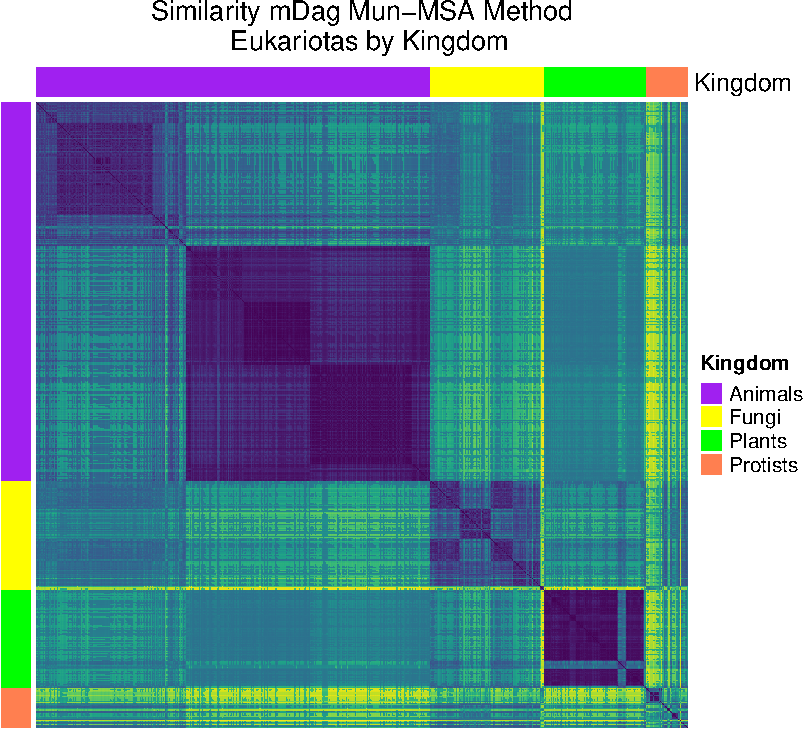
\includegraphics[width=0.3\textwidth,height=\textheight]{index_files/figure-pdf/unnamed-chunk-15-1.pdf}

}

\end{figure}

\hypertarget{mdag-global-core-for-eukaryotes}{%
\section*{mDag Global core for
eukaryotes}\label{mdag-global-core-for-eukaryotes}}
\addcontentsline{toc}{section}{mDag Global core for eukaryotes}

\markright{mDag Global core for eukaryotes}

Note that the mDAG core is empty as it does not contain any reactions.

\hypertarget{core-mdag}{%
\subsection*{Core mDAG}\label{core-mdag}}
\addcontentsline{toc}{subsection}{Core mDAG}

\begin{Shaded}
\begin{Highlighting}[]
\NormalTok{graph\_core\_mDAG}\OtherTok{=}\FunctionTok{read.graph}\NormalTok{(}
  \FunctionTok{paste0}\NormalTok{(path\_exp,}\StringTok{"Global/core/core\_mDAG.graphml"}\NormalTok{), }\AttributeTok{format =} \StringTok{"graphml"}\NormalTok{)}
\FunctionTok{summary}\NormalTok{(graph\_core\_mDAG)}
\end{Highlighting}
\end{Shaded}

\begin{verbatim}
IGRAPH c47f642 D--- 0 0 -- 
+ attr: color (v/c), label (v/c), id (v/c)
\end{verbatim}

\begin{Shaded}
\begin{Highlighting}[]
\NormalTok{knitr}\SpecialCharTok{::}\FunctionTok{include\_graphics}\NormalTok{(}
  \FunctionTok{paste0}\NormalTok{(path\_exp,}\StringTok{"Global/core/core\_mDAG.pdf"}\NormalTok{))}
\end{Highlighting}
\end{Shaded}

\begin{figure}[H]

{\centering \includegraphics[width=0.3\textwidth,height=\textheight]{data/results_ff15c187-62e7-37c2-96a7-c824f7eab671/data/Global/core/core_mDAG.pdf}

}

\caption{Core mDAG is empty}

\end{figure}

The graph core mDAG have 0 vertex and 0, is an empty graph.

\hypertarget{core-reaction-graph-rc}{%
\subsection*{Core reaction graph (RC)}\label{core-reaction-graph-rc}}
\addcontentsline{toc}{subsection}{Core reaction graph (RC)}

\begin{Shaded}
\begin{Highlighting}[]
\NormalTok{graph\_core\_RC}\OtherTok{=}\FunctionTok{read.graph}\NormalTok{(}
  \FunctionTok{paste0}\NormalTok{(path\_exp,}\StringTok{"Global/core/core\_RC.graphml"}\NormalTok{), }\AttributeTok{format =} \StringTok{"graphml"}\NormalTok{)}
\FunctionTok{summary}\NormalTok{(graph\_core\_mDAG)}
\end{Highlighting}
\end{Shaded}

\begin{verbatim}
IGRAPH c47f642 D--- 0 0 -- 
+ attr: color (v/c), label (v/c), id (v/c)
\end{verbatim}

\begin{Shaded}
\begin{Highlighting}[]
\NormalTok{knitr}\SpecialCharTok{::}\FunctionTok{include\_graphics}\NormalTok{(}
  \FunctionTok{paste0}\NormalTok{(path\_exp,}\StringTok{"Global/core/core\_RC.pdf"}\NormalTok{))}
\end{Highlighting}
\end{Shaded}

\begin{figure}[H]

{\centering \includegraphics[width=0.3\textwidth,height=\textheight]{data/results_ff15c187-62e7-37c2-96a7-c824f7eab671/data/Global/core/core_RC.pdf}

}

\caption{Core mDAG is empty}

\end{figure}

The graph core reaction graph have 0 vertex and 0, is an empty graph.

\hypertarget{mdag-global-pan-for-eukaryotes}{%
\section*{mDag Global pan for
eukaryotes}\label{mdag-global-pan-for-eukaryotes}}
\addcontentsline{toc}{section}{mDag Global pan for eukaryotes}

\markright{mDag Global pan for eukaryotes}

\hypertarget{pan-mdag}{%
\subsection*{Pan mDAG}\label{pan-mdag}}
\addcontentsline{toc}{subsection}{Pan mDAG}

\begin{Shaded}
\begin{Highlighting}[]
\NormalTok{graph\_pan\_mDAG}\OtherTok{=}\FunctionTok{read.graph}\NormalTok{(}
  \FunctionTok{paste0}\NormalTok{(path\_exp,}\StringTok{"TaxonomyLevels/Kingdom/Animals/pan/Animals\_pan\_mDAG.graphml"}\NormalTok{), }\AttributeTok{format =} \StringTok{"graphml"}\NormalTok{)}
\FunctionTok{summary}\NormalTok{(graph\_pan\_mDAG)}
\end{Highlighting}
\end{Shaded}

\begin{verbatim}
IGRAPH c49f6d2 D--- 1184 1261 -- 
+ attr: color (v/c), label (v/c), id (v/c), id (e/c)
\end{verbatim}

The graph pan mDAG have 1184 vertex and 1261.

\hypertarget{pan-reaction-graph-rc}{%
\subsection*{Pan Reaction graph (RC)}\label{pan-reaction-graph-rc}}
\addcontentsline{toc}{subsection}{Pan Reaction graph (RC)}

\begin{Shaded}
\begin{Highlighting}[]
\NormalTok{graph\_pan\_RC}\OtherTok{=}\FunctionTok{read.graph}\NormalTok{(}
  \FunctionTok{paste0}\NormalTok{(path\_exp,}\StringTok{"TaxonomyLevels/Kingdom/Animals/pan/Animals\_pan\_RC.graphml"}\NormalTok{), }\AttributeTok{format =} \StringTok{"graphml"}\NormalTok{)}
\FunctionTok{summary}\NormalTok{(graph\_pan\_RC)}
\end{Highlighting}
\end{Shaded}

\begin{verbatim}
IGRAPH c4abfa6 D--- 4556 5798 -- 
+ attr: color (v/c), label (v/c), id (v/c), id (e/c)
\end{verbatim}

The graph pan reaction graph have 4556 vertex and
\texttt{r}igraph::ecount(graph\_pan\_RC)`.

\begin{Shaded}
\begin{Highlighting}[]
\NormalTok{compo}\OtherTok{=}\FunctionTok{components}\NormalTok{(graph\_mDAG,}\AttributeTok{mode =} \StringTok{"weak"}\NormalTok{)}
\FunctionTok{str}\NormalTok{(compo)}
\end{Highlighting}
\end{Shaded}

\begin{verbatim}
List of 3
 $ membership: num [1:1026] 1 1 1 1 1 1 1 1 1 1 ...
 $ csize     : num [1:167] 589 1 1 1 1 1 4 3 4 3 ...
 $ no        : int 167
\end{verbatim}

\begin{Shaded}
\begin{Highlighting}[]
\NormalTok{compo}\SpecialCharTok{$}\NormalTok{csize}
\end{Highlighting}
\end{Shaded}

\begin{verbatim}
  [1] 589   1   1   1   1   1   4   3   4   3   2   3   3   1   1   1   2   6
 [19]   3   1   3   6   1   1   1   1   1   3   1   6   2   1   1   1   2   1
 [37]   1  14   1  16   1   6   2   2   4   1   1   1   1   1   1   1   1   1
 [55]  13   1   1   1   1   2   6   5   5   2   2  10   1   1   1   2   2   1
 [73]   1   1  62   6   2   1   2   1   1   1   2   1   2  14   3   1   1   1
 [91]   1   1   1   1   1   1   3   6   1   3   1   3   2   1   1   1   2   2
[109]   3   1   1   2   5   1   1   2   3   2   1   1   2   3   4   1   1   2
[127]   1   1   2   1   1   1   1   1   3   1   2   2   1   6   1   1   1   2
[145]   1   1   1   1   1   2   7   1  15   3   1   1   1   1   2   1   3   1
[163]   1   1   1   1   2
\end{verbatim}

\begin{Shaded}
\begin{Highlighting}[]
\NormalTok{k}\OtherTok{=}\FunctionTok{which.max}\NormalTok{(compo}\SpecialCharTok{$}\NormalTok{csize}\SpecialCharTok{==}\FunctionTok{max}\NormalTok{(compo}\SpecialCharTok{$}\NormalTok{csize))}
\NormalTok{k}
\end{Highlighting}
\end{Shaded}

\begin{verbatim}
[1] 1
\end{verbatim}

\begin{Shaded}
\begin{Highlighting}[]
\FunctionTok{table}\NormalTok{(compo}\SpecialCharTok{$}\NormalTok{membership)}
\end{Highlighting}
\end{Shaded}

\begin{verbatim}

  1   2   3   4   5   6   7   8   9  10  11  12  13  14  15  16  17  18  19  20 
589   1   1   1   1   1   4   3   4   3   2   3   3   1   1   1   2   6   3   1 
 21  22  23  24  25  26  27  28  29  30  31  32  33  34  35  36  37  38  39  40 
  3   6   1   1   1   1   1   3   1   6   2   1   1   1   2   1   1  14   1  16 
 41  42  43  44  45  46  47  48  49  50  51  52  53  54  55  56  57  58  59  60 
  1   6   2   2   4   1   1   1   1   1   1   1   1   1  13   1   1   1   1   2 
 61  62  63  64  65  66  67  68  69  70  71  72  73  74  75  76  77  78  79  80 
  6   5   5   2   2  10   1   1   1   2   2   1   1   1  62   6   2   1   2   1 
 81  82  83  84  85  86  87  88  89  90  91  92  93  94  95  96  97  98  99 100 
  1   1   2   1   2  14   3   1   1   1   1   1   1   1   1   1   3   6   1   3 
101 102 103 104 105 106 107 108 109 110 111 112 113 114 115 116 117 118 119 120 
  1   3   2   1   1   1   2   2   3   1   1   2   5   1   1   2   3   2   1   1 
121 122 123 124 125 126 127 128 129 130 131 132 133 134 135 136 137 138 139 140 
  2   3   4   1   1   2   1   1   2   1   1   1   1   1   3   1   2   2   1   6 
141 142 143 144 145 146 147 148 149 150 151 152 153 154 155 156 157 158 159 160 
  1   1   1   2   1   1   1   1   1   2   7   1  15   3   1   1   1   1   2   1 
161 162 163 164 165 166 167 
  3   1   1   1   1   1   2 
\end{verbatim}

\begin{Shaded}
\begin{Highlighting}[]
\NormalTok{vertex}\OtherTok{=}\FunctionTok{which}\NormalTok{(compo}\SpecialCharTok{$}\NormalTok{membership}\SpecialCharTok{==}\NormalTok{k)}
\FunctionTok{length}\NormalTok{(vertex)}
\end{Highlighting}
\end{Shaded}

\begin{verbatim}
[1] 589
\end{verbatim}

\begin{Shaded}
\begin{Highlighting}[]
\NormalTok{Big\_Component}\OtherTok{=}\FunctionTok{induced\_subgraph}\NormalTok{(graph\_mDAG, }\AttributeTok{vids=}\NormalTok{vertex)}
\NormalTok{igraph}\SpecialCharTok{::}\FunctionTok{vcount}\NormalTok{(Big\_Component)}
\end{Highlighting}
\end{Shaded}

\begin{verbatim}
[1] 589
\end{verbatim}

\begin{Shaded}
\begin{Highlighting}[]
\NormalTok{igraph}\SpecialCharTok{::}\FunctionTok{ecount}\NormalTok{(Big\_Component)}
\end{Highlighting}
\end{Shaded}

\begin{verbatim}
[1] 774
\end{verbatim}

The curated plot of the bigger component of hsa mDAG

\begin{Shaded}
\begin{Highlighting}[]
\NormalTok{knitr}\SpecialCharTok{::}\FunctionTok{include\_graphics}\NormalTok{(}\FunctionTok{paste0}\NormalTok{(path\_exp,}
                               \StringTok{"Individuals/hsa/hsa\_mDAG\_biggerDAG.pdf"}\NormalTok{))}
\end{Highlighting}
\end{Shaded}

\begin{figure}[H]

{\centering 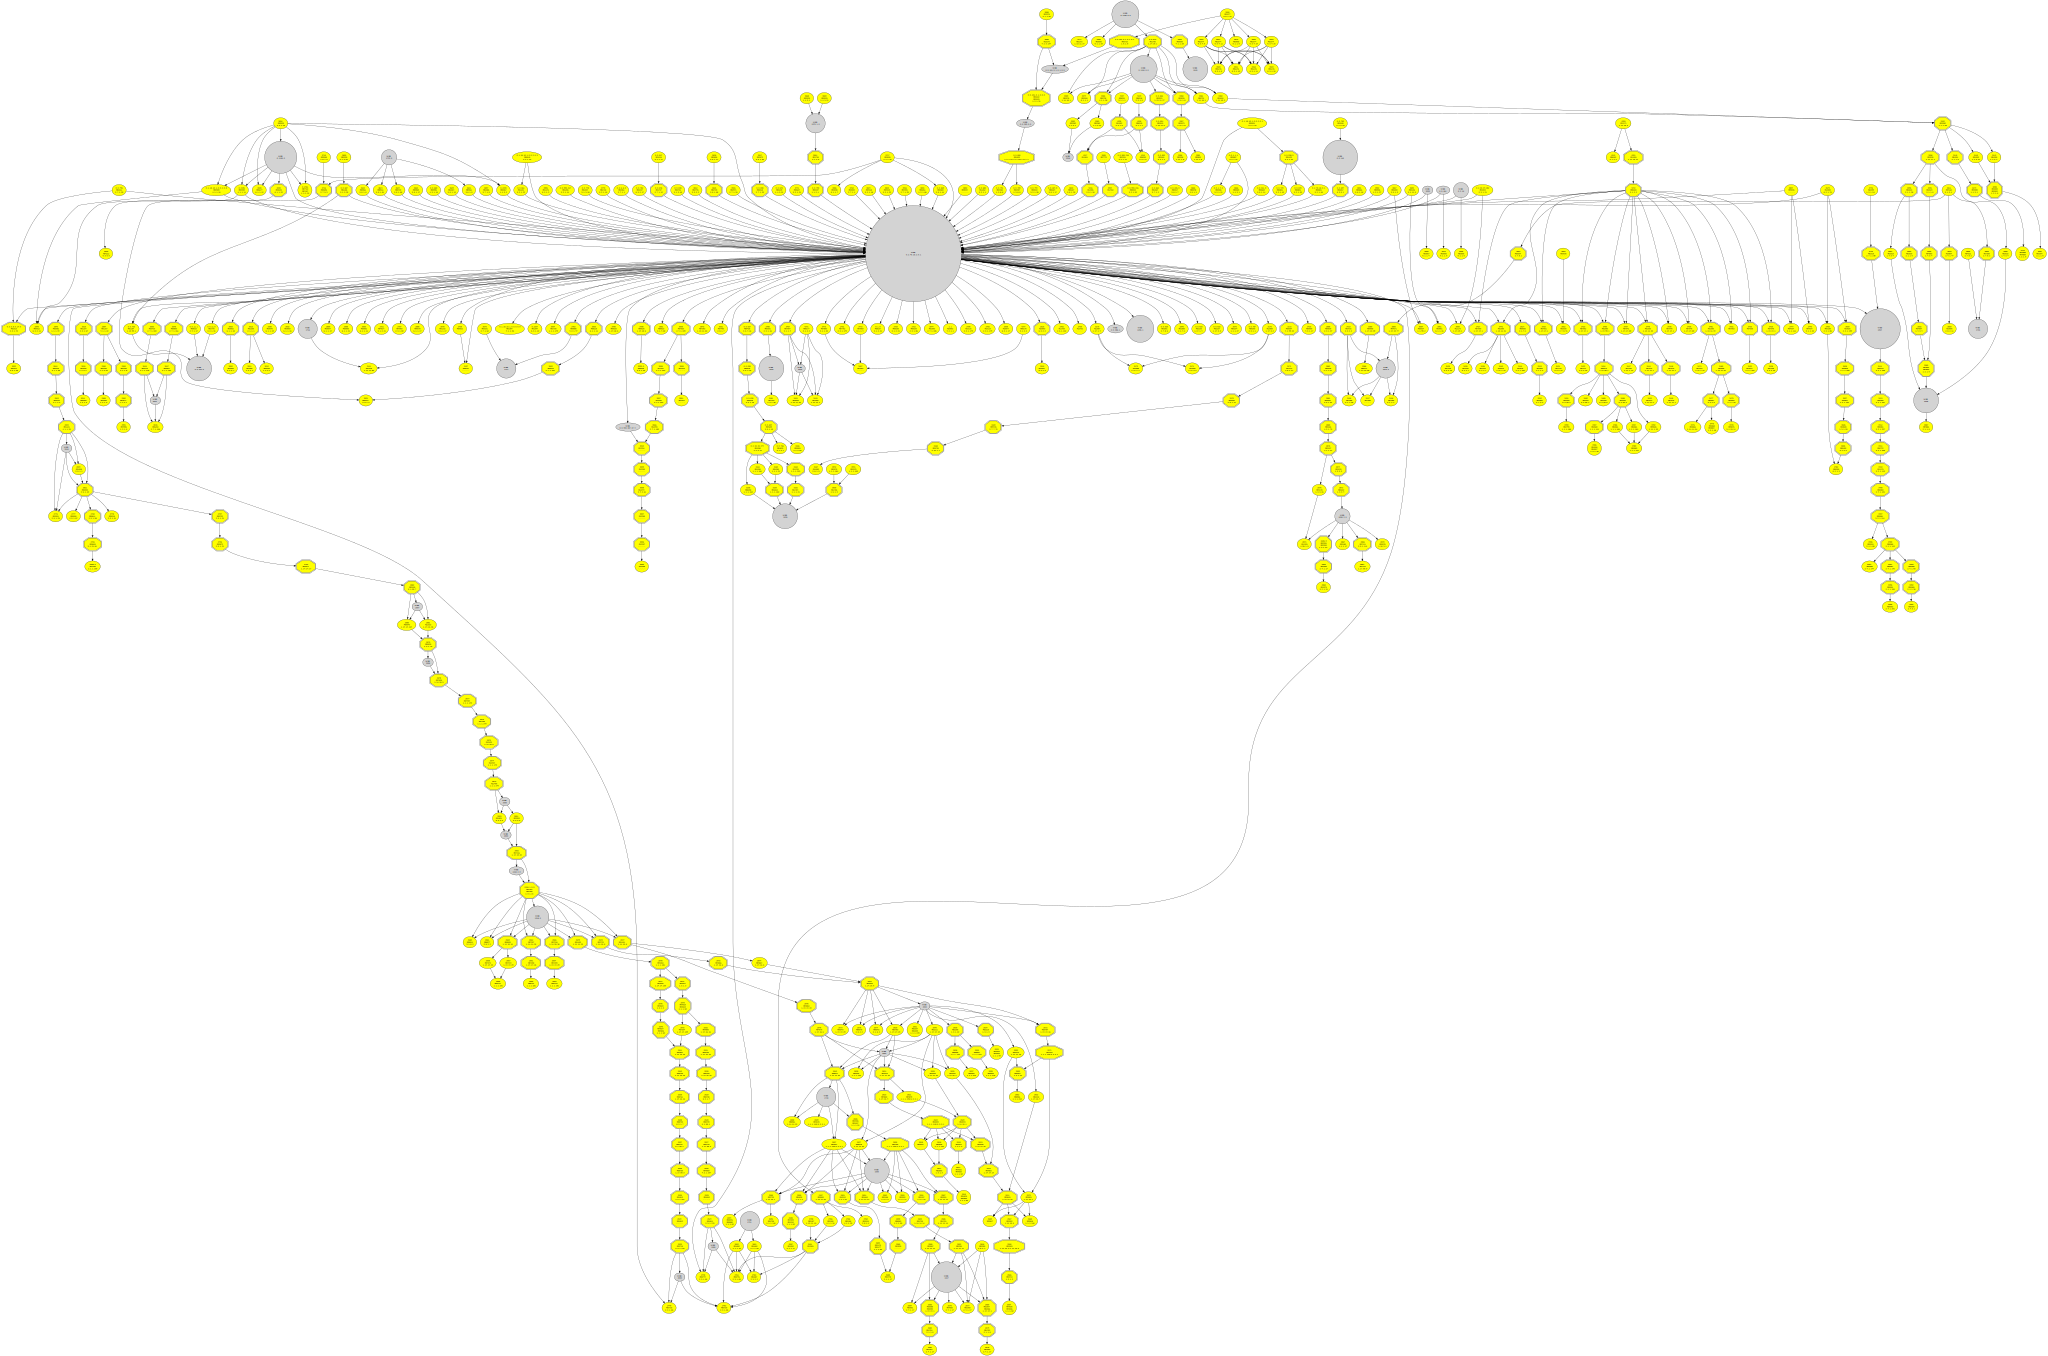
\includegraphics[width=0.3\textwidth,height=\textheight]{data/results_ff15c187-62e7-37c2-96a7-c824f7eab671/data/Individuals/hsa/hsa_mDAG_biggerDAG.pdf}

}

\end{figure}

\bookmarksetup{startatroot}

\hypertarget{similarities-and-metadata-for-an-experiment}{%
\chapter*{Similarities and metadata for an
experiment}\label{similarities-and-metadata-for-an-experiment}}
\addcontentsline{toc}{chapter}{Similarities and metadata for an
experiment}

\markboth{Similarities and metadata for an experiment}{Similarities and
metadata for an experiment}

We will first load the metadata and adapt them to the structure of the
similarities to facilitate the creation of the graphs and statistics.

Remenber de path of the experiment:

\begin{Shaded}
\begin{Highlighting}[]
\NormalTok{path\_exp}
\end{Highlighting}
\end{Shaded}

\begin{verbatim}
[1] "data/results_ff15c187-62e7-37c2-96a7-c824f7eab671/data/"
\end{verbatim}

\hypertarget{load-meta-data-from-eukariotes-experimet}{%
\section*{Load meta data from eukariotes
experimet}\label{load-meta-data-from-eukariotes-experimet}}
\addcontentsline{toc}{section}{Load meta data from eukariotes experimet}

\markright{Load meta data from eukariotes experimet}

Meta data mDa\_Id and taxonomy sort by Kingdom,Filum,Class,mDAG\_Id

\begin{Shaded}
\begin{Highlighting}[]
\NormalTok{path\_exp}
\end{Highlighting}
\end{Shaded}

\begin{verbatim}
[1] "data/results_ff15c187-62e7-37c2-96a7-c824f7eab671/data/"
\end{verbatim}

\begin{Shaded}
\begin{Highlighting}[]
\NormalTok{Results}\OtherTok{=}\FunctionTok{read\_csv}\NormalTok{(}\FunctionTok{paste0}\NormalTok{(path\_exp,}\StringTok{"Results.csv"}\NormalTok{))}
\FunctionTok{names}\NormalTok{(Results)[}\FunctionTok{c}\NormalTok{(}\DecValTok{1}\NormalTok{,}\DecValTok{3}\NormalTok{,}\DecValTok{4}\NormalTok{)]}\OtherTok{=}\FunctionTok{c}\NormalTok{(}\StringTok{"Organism"}\NormalTok{,}\StringTok{"mDAG\_Id"}\NormalTok{,}\StringTok{"Full\_Name"}\NormalTok{)}
\CommentTok{\#code=Results \%\textgreater{}\% select(Organism:mDAG\_Id)}
\NormalTok{taxo}\OtherTok{=}\NormalTok{Results }\SpecialCharTok{\%\textgreater{}\%} \FunctionTok{select}\NormalTok{(Organism}\SpecialCharTok{:}\NormalTok{Full\_Name)}
\NormalTok{index}\OtherTok{=}\FunctionTok{is.na}\NormalTok{(taxo}\SpecialCharTok{$}\NormalTok{Categories)}
\NormalTok{taxo}\OtherTok{=}\NormalTok{taxo }\SpecialCharTok{\%\textgreater{}\%} \FunctionTok{separate}\NormalTok{(Categories,}\AttributeTok{into=}\FunctionTok{c}\NormalTok{(}\StringTok{"Kingdom"}\NormalTok{,}\StringTok{"Phylum"}\NormalTok{,}\StringTok{"Class"}\NormalTok{))}
\NormalTok{taxo}\SpecialCharTok{$}\NormalTok{Class[index]}\OtherTok{=}\FunctionTok{paste}\NormalTok{(taxo}\SpecialCharTok{$}\NormalTok{Kingdom[index],taxo}\SpecialCharTok{$}\NormalTok{Phylum[index])}
\NormalTok{meta\_taxo}\OtherTok{=}\NormalTok{taxo }\SpecialCharTok{\%\textgreater{}\%} \FunctionTok{arrange}\NormalTok{(Kingdom,Phylum)}
\NormalTok{index}\OtherTok{=}\FunctionTok{which}\NormalTok{(}\FunctionTok{is.na}\NormalTok{(meta\_taxo}\SpecialCharTok{$}\NormalTok{Class))}
\NormalTok{meta\_taxo}\SpecialCharTok{$}\NormalTok{Class[index]}\OtherTok{=}\NormalTok{meta\_taxo}\SpecialCharTok{$}\NormalTok{Phylum[index]}
\NormalTok{aux}\OtherTok{=}\FunctionTok{table}\NormalTok{(meta\_taxo}\SpecialCharTok{$}\NormalTok{Class)}
\NormalTok{freq}\OtherTok{=}\FunctionTok{tibble}\NormalTok{(}\AttributeTok{Class=}\FunctionTok{names}\NormalTok{(aux),}\AttributeTok{Freq\_Class=}\NormalTok{aux)}
\FunctionTok{names}\NormalTok{(freq)}\OtherTok{=}\FunctionTok{c}\NormalTok{(}\StringTok{"Class"}\NormalTok{,}\StringTok{"Freq\_Class"}\NormalTok{)}
\NormalTok{meta\_taxo }\OtherTok{=}\NormalTok{meta\_taxo }\SpecialCharTok{\%\textgreater{}\%} \FunctionTok{left\_join}\NormalTok{(freq)}\SpecialCharTok{\%\textgreater{}\%}
  \FunctionTok{arrange}\NormalTok{(Kingdom,Phylum,}\FunctionTok{desc}\NormalTok{(Freq\_Class))}
\FunctionTok{head}\NormalTok{(meta\_taxo)}
\end{Highlighting}
\end{Shaded}

\begin{verbatim}
# A tibble: 6 x 7
  Organism Kingdom Phylum     Class    mDAG_Id Full_Name              Freq_Class
  <chr>    <chr>   <chr>      <chr>    <chr>   <chr>                  <table[1d>
1 hro      Animals Annelids   Annelids 0576    Helobdella robusta       1       
2 aag      Animals Arthropods Insects  0035    Aedes aegypti (yellow~ 130       
3 aalb     Animals Arthropods Insects  0276    Aedes albopictus (Asi~ 130       
4 aali     Animals Arthropods Insects  0267    Anopheles albimanus    130       
5 aara     Animals Arthropods Insects  0362    Anopheles arabiensis   130       
6 acep     Animals Arthropods Insects  0054    Atta cephalotes (leaf~ 130       
\end{verbatim}

\begin{Shaded}
\begin{Highlighting}[]
\FunctionTok{table}\NormalTok{(meta\_taxo}\SpecialCharTok{$}\NormalTok{Kingdom) }\SpecialCharTok{\%\textgreater{}\%}\NormalTok{ kable }\SpecialCharTok{\%\textgreater{}\%}
  \FunctionTok{kable\_styling}\NormalTok{(}\StringTok{"striped"}\NormalTok{, }\AttributeTok{full\_width =}\NormalTok{ F,}\AttributeTok{position=}\StringTok{"left"}\NormalTok{)}\SpecialCharTok{\%\textgreater{}\%} 
 \FunctionTok{scroll\_box}\NormalTok{(}\AttributeTok{width =} \StringTok{"400px"}\NormalTok{, }\AttributeTok{height =} \StringTok{"200px"}\NormalTok{)}
\end{Highlighting}
\end{Shaded}

\begin{tabular}{l|r}
\hline
Var1 & Freq\\
\hline
Animals & 535\\
\hline
Fungi & 154\\
\hline
Plants & 139\\
\hline
Protists & 56\\
\hline
\end{tabular}

\begin{Shaded}
\begin{Highlighting}[]
\FunctionTok{table}\NormalTok{(meta\_taxo}\SpecialCharTok{$}\NormalTok{Phylum,meta\_taxo}\SpecialCharTok{$}\NormalTok{Kingdom) }\SpecialCharTok{\%\textgreater{}\%}\NormalTok{ kable }\SpecialCharTok{\%\textgreater{}\%}
  \FunctionTok{kable\_styling}\NormalTok{(}\StringTok{"striped"}\NormalTok{, }\AttributeTok{full\_width =}\NormalTok{ F,}\AttributeTok{position=}\StringTok{"left"}\NormalTok{)}\SpecialCharTok{\%\textgreater{}\%} 
 \FunctionTok{scroll\_box}\NormalTok{(}\AttributeTok{width =} \StringTok{"500px"}\NormalTok{, }\AttributeTok{height =} \StringTok{"500px"}\NormalTok{)}
\end{Highlighting}
\end{Shaded}

\begin{tabular}{l|r|r|r|r}
\hline
  & Animals & Fungi & Plants & Protists\\
\hline
Alveolates & 0 & 0 & 0 & 25\\
\hline
Amoebozoa & 0 & 0 & 0 & 7\\
\hline
Annelids & 1 & 0 & 0 & 0\\
\hline
Arthropods & 158 & 0 & 0 & 0\\
\hline
Ascomycetes & 0 & 113 & 0 & 0\\
\hline
Basal & 0 & 0 & 2 & 0\\
\hline
Basidiomycetes & 0 & 36 & 0 & 0\\
\hline
Brachiopodas & 1 & 0 & 0 & 0\\
\hline
Cephalochordates & 2 & 0 & 0 & 0\\
\hline
Choanoflagellates & 0 & 0 & 0 & 2\\
\hline
Cnidarians & 10 & 0 & 0 & 0\\
\hline
Cryptomonads & 0 & 0 & 0 & 1\\
\hline
Echinoderms & 3 & 0 & 0 & 0\\
\hline
Eudicots & 0 & 0 & 98 & 0\\
\hline
Euglenozoa & 0 & 0 & 0 & 9\\
\hline
Ferns & 0 & 0 & 1 & 0\\
\hline
Flatworms & 4 & 0 & 0 & 0\\
\hline
Green & 0 & 0 & 11 & 0\\
\hline
Haptophyta & 0 & 0 & 0 & 1\\
\hline
Hemichordates & 1 & 0 & 0 & 0\\
\hline
Heterolobosea & 0 & 0 & 0 & 1\\
\hline
Metamonada & 0 & 0 & 0 & 2\\
\hline
Microsporidians & 0 & 5 & 0 & 0\\
\hline
Mollusks & 14 & 0 & 0 & 0\\
\hline
Monocots & 0 & 0 & 23 & 0\\
\hline
Mosses & 0 & 0 & 1 & 0\\
\hline
Nematodes & 6 & 0 & 0 & 0\\
\hline
Placozoans & 1 & 0 & 0 & 0\\
\hline
Poriferans & 1 & 0 & 0 & 0\\
\hline
Red & 0 & 0 & 3 & 0\\
\hline
Stramenopiles & 0 & 0 & 0 & 8\\
\hline
Tunicates & 2 & 0 & 0 & 0\\
\hline
Vertebrates & 331 & 0 & 0 & 0\\
\hline
\end{tabular}

\bookmarksetup{startatroot}

\hypertarget{similarities-msamunkres-methods}{%
\chapter*{Similarities MSA,Munkres
methods}\label{similarities-msamunkres-methods}}
\addcontentsline{toc}{chapter}{Similarities MSA,Munkres methods}

\markboth{Similarities MSA,Munkres methods}{Similarities MSA,Munkres
methods}

In this section we will show the similarities between mDAG's using
different methods.

The experiment data set consists of 884 eurkaryotes from the animal,
plant, fungus, and protist kingdoms.

\begin{tabular}{l|r}
\hline
Kingdom & Abs. Freq.\\
\hline
Animals & 535\\
\hline
Fungi & 154\\
\hline
Plants & 139\\
\hline
Protists & 56\\
\hline
\end{tabular}

\begin{Shaded}
\begin{Highlighting}[]
\NormalTok{list\_Sim}\OtherTok{=}\FunctionTok{dir}\NormalTok{(path\_exp,}\AttributeTok{pattern=}\StringTok{"\^{}Similarities"}\NormalTok{)}
\NormalTok{list\_Sim}
\end{Highlighting}
\end{Shaded}

\begin{verbatim}
[1] "Similarities_MBB_MSAMethod.csv"      "Similarities_MBB_MunkresMethod.csv" 
[3] "Similarities_mDAG_MSAMethod.csv"     "Similarities_mDAG_MunkresMethod.csv"
[5] "Similarities_mDAGOnReaction.csv"    
\end{verbatim}

Load MDAG similarities

\begin{Shaded}
\begin{Highlighting}[]
\NormalTok{Sim\_MSA\_mDAG}\OtherTok{=}\FunctionTok{read\_csv}\NormalTok{(}\FunctionTok{paste0}\NormalTok{(path\_exp,}
                             \StringTok{"Similarities\_mDAG\_MSAMethod.csv"}\NormalTok{))}
\NormalTok{Sim\_MSA\_mDAG}\OtherTok{=}\FunctionTok{as.matrix}\NormalTok{(Sim\_MSA\_mDAG[,}\SpecialCharTok{{-}}\DecValTok{1}\NormalTok{])}
\FunctionTok{rownames}\NormalTok{(Sim\_MSA\_mDAG)}\OtherTok{=}\FunctionTok{colnames}\NormalTok{(Sim\_MSA\_mDAG)}
\NormalTok{Sim\_MSA\_mDAG}\OtherTok{=}\NormalTok{Sim\_MSA\_mDAG[meta\_taxo}\SpecialCharTok{$}\NormalTok{mDAG\_Id,meta\_taxo}\SpecialCharTok{$}\NormalTok{mDAG\_Id]}
\end{Highlighting}
\end{Shaded}

\begin{Shaded}
\begin{Highlighting}[]
\NormalTok{Sim\_Mun\_mDAG}\OtherTok{=}\FunctionTok{read\_csv}\NormalTok{(}\FunctionTok{paste0}\NormalTok{(path\_exp,}
\StringTok{"Similarities\_mDAG\_MunkresMethod.csv"}\NormalTok{))}
\NormalTok{Sim\_Mun\_mDAG}\OtherTok{=}\FunctionTok{as.matrix}\NormalTok{(Sim\_Mun\_mDAG[,}\SpecialCharTok{{-}}\DecValTok{1}\NormalTok{])}
\FunctionTok{rownames}\NormalTok{(Sim\_Mun\_mDAG)}\OtherTok{=}\FunctionTok{colnames}\NormalTok{(Sim\_Mun\_mDAG)}
\NormalTok{Sim\_Mun\_mDAG}\OtherTok{=}\NormalTok{Sim\_Mun\_mDAG[meta\_taxo}\SpecialCharTok{$}\NormalTok{mDAG\_Id,meta\_taxo}\SpecialCharTok{$}\NormalTok{mDAG\_Id]}
\end{Highlighting}
\end{Shaded}

\hypertarget{heatmaps}{%
\section*{Heatmaps}\label{heatmaps}}
\addcontentsline{toc}{section}{Heatmaps}

\markright{Heatmaps}

\hypertarget{heatmap-similarity-msa-method}{%
\subsection*{Heatmap Similarity MSA
method}\label{heatmap-similarity-msa-method}}
\addcontentsline{toc}{subsection}{Heatmap Similarity MSA method}

\begin{Shaded}
\begin{Highlighting}[]
\NormalTok{dff}\OtherTok{\textless{}{-}}\NormalTok{meta\_taxo }\SpecialCharTok{\%\textgreater{}\%} \FunctionTok{select}\NormalTok{(Kingdom)  }\SpecialCharTok{\%\textgreater{}\%} \FunctionTok{as.data.frame}\NormalTok{()}
\CommentTok{\#str(dff)}

\NormalTok{colorsK }\OtherTok{\textless{}{-}} \FunctionTok{list}\NormalTok{(}\AttributeTok{Kingdom=} \FunctionTok{c}\NormalTok{(}\StringTok{"Animals"}\OtherTok{=}\StringTok{"red"}\NormalTok{,}
                           \StringTok{"Plants"}\OtherTok{=}\StringTok{"green"}\NormalTok{,}
                           \StringTok{"Fungi"}\OtherTok{=}\StringTok{"yellow"}\NormalTok{,}
                           \StringTok{"Protists"}\OtherTok{=}\StringTok{"black"}\NormalTok{))}

\NormalTok{anot }\OtherTok{\textless{}{-}} \FunctionTok{HeatmapAnnotation}\NormalTok{(}\AttributeTok{df=}\NormalTok{dff, }\AttributeTok{col =}\NormalTok{ colorsK)}

\CommentTok{\#S=Sim\_MSA\_mDAG}

\NormalTok{MSA\_heat\_1 }\OtherTok{\textless{}{-}} \FunctionTok{Heatmap}\NormalTok{(}\AttributeTok{matrix =}\NormalTok{ Sim\_MSA\_mDAG, }
                          \AttributeTok{column\_title=}\StringTok{"m{-}DAGs MSA{-}similarity }\SpecialCharTok{\textbackslash{}n}\StringTok{  Eukaryotes by Kingdom"}\NormalTok{,}
            \AttributeTok{name =} \StringTok{"Kingdom"}\NormalTok{,}
            \AttributeTok{heatmap\_legend\_param =} \FunctionTok{list}\NormalTok{(}
    \AttributeTok{at =} \FunctionTok{c}\NormalTok{(}\FloatTok{0.4}\NormalTok{,}\FloatTok{0.5}\NormalTok{,}\FloatTok{0.6}\NormalTok{,}\FloatTok{0.7}\NormalTok{,}\FloatTok{0.8}\NormalTok{,}\FloatTok{0.9}\NormalTok{,}\DecValTok{1}\NormalTok{)),}
        \AttributeTok{col=}\FunctionTok{rev}\NormalTok{(}\FunctionTok{viridis}\NormalTok{(}\DecValTok{256}\NormalTok{)),}
        \AttributeTok{cluster\_rows =} \ConstantTok{FALSE}\NormalTok{,}
        \AttributeTok{cluster\_columns =} \ConstantTok{FALSE}\NormalTok{,}
        \AttributeTok{top\_annotation =}\NormalTok{ anot,}
        \AttributeTok{show\_column\_names =} \ConstantTok{FALSE}\NormalTok{, }
        \AttributeTok{show\_row\_names =} \ConstantTok{FALSE}\NormalTok{,}
        \AttributeTok{left\_annotation =} \FunctionTok{rowAnnotation}\NormalTok{(}\AttributeTok{df =}\NormalTok{ dff,                                    }\AttributeTok{col=}\NormalTok{colorsK,}\AttributeTok{show\_annotation\_name=}\ConstantTok{FALSE}\NormalTok{))}
  
\FunctionTok{draw}\NormalTok{(MSA\_heat\_1, }\AttributeTok{merge\_legend =} \ConstantTok{TRUE}\NormalTok{)}
\end{Highlighting}
\end{Shaded}

\begin{figure}[H]

{\centering \includegraphics[width=0.3\textwidth,height=\textheight]{index_files/figure-pdf/unnamed-chunk-31-1.pdf}

}

\end{figure}

\begin{Shaded}
\begin{Highlighting}[]
\NormalTok{meta\_animals}\OtherTok{=}\NormalTok{ meta\_taxo }\SpecialCharTok{\%\textgreater{}\%} \FunctionTok{filter}\NormalTok{(Kingdom}\SpecialCharTok{==}\StringTok{"Animals"}\NormalTok{)}
\NormalTok{nombres}\OtherTok{=}\FunctionTok{unique}\NormalTok{(meta\_animals}\SpecialCharTok{$}\NormalTok{Phylum)}
\NormalTok{aux\_order}\OtherTok{=}\FunctionTok{table}\NormalTok{(meta\_animals}\SpecialCharTok{$}\NormalTok{Phylum)}
\NormalTok{dff}\OtherTok{\textless{}{-}}\NormalTok{meta\_taxo }\SpecialCharTok{\%\textgreater{}\%} \FunctionTok{filter}\NormalTok{(Kingdom}\SpecialCharTok{==}\StringTok{"Animals"}\NormalTok{) }\SpecialCharTok{\%\textgreater{}\%} \FunctionTok{select}\NormalTok{(Phylum) }\SpecialCharTok{\%\textgreater{}\%} \FunctionTok{as.data.frame}\NormalTok{()}
\CommentTok{\#str(dff)}
\NormalTok{nombres}\OtherTok{=}\FunctionTok{unique}\NormalTok{(dff}\SpecialCharTok{$}\NormalTok{Phylum)}
\NormalTok{col}\OtherTok{=}\FunctionTok{rainbow}\NormalTok{(}\FunctionTok{length}\NormalTok{(nombres))}
\NormalTok{colorsP}\OtherTok{=}\FunctionTok{list}\NormalTok{(}\AttributeTok{Phylum=}\NormalTok{col)}
\FunctionTok{names}\NormalTok{(colorsP}\SpecialCharTok{$}\NormalTok{Phylum)}\OtherTok{=}\NormalTok{nombres}

\NormalTok{anotation\_MSA\_H2 }\OtherTok{\textless{}{-}} \FunctionTok{HeatmapAnnotation}\NormalTok{(}\AttributeTok{df=}\NormalTok{dff, }\AttributeTok{col =}\NormalTok{ colorsP,}\AttributeTok{show\_legend =} \ConstantTok{TRUE}\NormalTok{)}

\CommentTok{\#orderP\_freq=sort(table(dff$Phylum),decreasing = TRUE)}
\CommentTok{\#orderP\_freq=tibble(Phylum=names(orderP\_freq),Freq=orderP\_freq)}

\NormalTok{MSA\_heat\_2 }\OtherTok{\textless{}{-}} \FunctionTok{Heatmap}\NormalTok{(}\AttributeTok{matrix =}\NormalTok{ Sim\_MSA\_mDAG[}\DecValTok{1}\SpecialCharTok{:}\DecValTok{535}\NormalTok{,}\DecValTok{1}\SpecialCharTok{:}\DecValTok{535}\NormalTok{], }
              \AttributeTok{column\_title=}\StringTok{"m{-}DAGs MSA{-}similarity }\SpecialCharTok{\textbackslash{}n}\StringTok{  Animal  Phyla"}\NormalTok{,}
            \AttributeTok{name =} \StringTok{" "}\NormalTok{, }
            \AttributeTok{heatmap\_legend\_param =} \FunctionTok{list}\NormalTok{(}\AttributeTok{at =} \FunctionTok{seq}\NormalTok{(}\DecValTok{0}\NormalTok{,}\DecValTok{1}\NormalTok{,}\AttributeTok{by=}\FloatTok{0.1}\NormalTok{)),}
        \AttributeTok{col=}\FunctionTok{rev}\NormalTok{(}\FunctionTok{viridis}\NormalTok{(}\DecValTok{256}\NormalTok{)),}
        \AttributeTok{cluster\_rows =} \ConstantTok{FALSE}\NormalTok{,}
        \AttributeTok{cluster\_columns =} \ConstantTok{FALSE}\NormalTok{,}
        \AttributeTok{top\_annotation =}\NormalTok{ anotation\_MSA\_H2,}
        \AttributeTok{show\_column\_names =} \ConstantTok{FALSE}\NormalTok{, }
        \AttributeTok{show\_row\_names =} \ConstantTok{FALSE}\NormalTok{,}
        \AttributeTok{left\_annotation =} \FunctionTok{rowAnnotation}\NormalTok{(}\AttributeTok{df =}\NormalTok{ dff,                                    }\AttributeTok{col=}\NormalTok{colorsP,}\AttributeTok{show\_annotation\_name=}\ConstantTok{FALSE}\NormalTok{))}
  
\FunctionTok{draw}\NormalTok{(MSA\_heat\_2, }\AttributeTok{merge\_legend =} \ConstantTok{TRUE}\NormalTok{)}
\end{Highlighting}
\end{Shaded}

\begin{figure}[H]

{\centering \includegraphics[width=0.3\textwidth,height=\textheight]{index_files/figure-pdf/unnamed-chunk-32-1.pdf}

}

\end{figure}

\hypertarget{mds-multidimensional-scaling}{%
\section*{MDS (Multidimensional
Scaling)}\label{mds-multidimensional-scaling}}
\addcontentsline{toc}{section}{MDS (Multidimensional Scaling)}

\markright{MDS (Multidimensional Scaling)}

\begin{Shaded}
\begin{Highlighting}[]
\DocumentationTok{\#\# Metric multidimensional scaling (mMDS)}
\NormalTok{mds7 }\OtherTok{\textless{}{-}} \FunctionTok{cmdscale}\NormalTok{(}\FunctionTok{sqrt}\NormalTok{(}\DecValTok{1}\SpecialCharTok{{-}}\NormalTok{Sim\_MSA\_mDAG}\SpecialCharTok{\^{}}\DecValTok{2}\NormalTok{),}\AttributeTok{k=}\DecValTok{7}\NormalTok{,}\AttributeTok{eig=}\ConstantTok{TRUE}\NormalTok{)}
\CommentTok{\#pairs(mds7$points[,1:4])}
\NormalTok{mds7}\SpecialCharTok{$}\NormalTok{GOF}
\end{Highlighting}
\end{Shaded}

\begin{verbatim}
[1] 0.4406568 0.5541042
\end{verbatim}

\begin{Shaded}
\begin{Highlighting}[]
\NormalTok{mds }\OtherTok{\textless{}{-}}\NormalTok{ mds7}\SpecialCharTok{$}\NormalTok{points }\SpecialCharTok{\%\textgreater{}\%}  \FunctionTok{as\_tibble}\NormalTok{()}
\FunctionTok{colnames}\NormalTok{(mds) }\OtherTok{\textless{}{-}}\FunctionTok{paste0}\NormalTok{(}\StringTok{"Dim."}\NormalTok{,}\DecValTok{1}\SpecialCharTok{:}\FunctionTok{dim}\NormalTok{(mds7}\SpecialCharTok{$}\NormalTok{points)[}\DecValTok{2}\NormalTok{])}


\NormalTok{cooordinates}\OtherTok{=}\FunctionTok{as\_tibble}\NormalTok{(mds7}\SpecialCharTok{$}\NormalTok{points)}
\FunctionTok{colnames}\NormalTok{(cooordinates)}\OtherTok{=}\FunctionTok{paste}\NormalTok{(}\StringTok{"Component"}\NormalTok{,}\DecValTok{1}\SpecialCharTok{:}\DecValTok{7}\NormalTok{)}
\FunctionTok{ggpairs}\NormalTok{(cooordinates,}\AttributeTok{columns=}\DecValTok{1}\SpecialCharTok{:}\DecValTok{4}\NormalTok{,}\FunctionTok{aes}\NormalTok{(}\AttributeTok{color=}\NormalTok{meta\_taxo}\SpecialCharTok{$}\NormalTok{Kingdom,}\AttributeTok{alpha=}\FloatTok{0.5}\NormalTok{,}\AttributeTok{title=}\StringTok{"MDS 4 dimensions projection"}\NormalTok{,}\AttributeTok{legend=}\DecValTok{1}\NormalTok{),}\AttributeTok{upper=}\FunctionTok{list}\NormalTok{(}\AttributeTok{continuous=}\StringTok{"points"}\NormalTok{)) }\SpecialCharTok{+}\FunctionTok{scale\_fill\_manual}\NormalTok{(}\AttributeTok{values =}\NormalTok{ colorsK}\SpecialCharTok{$}\NormalTok{Kingdom)}\SpecialCharTok{+} \FunctionTok{theme}\NormalTok{(}\AttributeTok{legend.position =} \StringTok{"left"}\NormalTok{)}
\end{Highlighting}
\end{Shaded}

\begin{figure}[H]

{\centering \includegraphics[width=0.3\textwidth,height=\textheight]{index_files/figure-pdf/unnamed-chunk-33-1.pdf}

}

\end{figure}

\begin{Shaded}
\begin{Highlighting}[]
\NormalTok{mds }\OtherTok{\textless{}{-}}\NormalTok{ mds }\SpecialCharTok{\%\textgreater{}\%}
  \FunctionTok{mutate}\NormalTok{(}\AttributeTok{groups =}\FunctionTok{as.factor}\NormalTok{(meta\_taxo}\SpecialCharTok{$}\NormalTok{Kingdom))}


\CommentTok{\#,text= \textasciitilde{}paste("Age:", groups, \textquotesingle{}\textless{}br\textgreater{}Name:\textquotesingle{})}
\FunctionTok{length}\NormalTok{(}\FunctionTok{unique}\NormalTok{(meta\_taxo}\SpecialCharTok{$}\NormalTok{Phylum))}
\end{Highlighting}
\end{Shaded}

\begin{verbatim}
[1] 33
\end{verbatim}

\begin{Shaded}
\begin{Highlighting}[]
\NormalTok{col\_mds}\OtherTok{=}\FunctionTok{rainbow}\NormalTok{(}\DecValTok{33}\NormalTok{)}


\CommentTok{\#col\_mds=c("purple","green","yellow","coral")}
\CommentTok{\#mcol\_mds=bremer.pal(7,"Greens")}

\CommentTok{\# fig \textless{}{-} }
\CommentTok{\# plot\_ly(}
\CommentTok{\#   mds, x = \textasciitilde{}Dim.1, y = \textasciitilde{}Dim.2,}
\CommentTok{\#   color = \textasciitilde{}groups, }
\CommentTok{\#   colors= colors,}
\CommentTok{\#   type="scatter",}
\CommentTok{\#   mode="markers") \%\textgreater{}\%}
\CommentTok{\#   layout(}
\CommentTok{\#     xaxis = list(autorange=2,}
\CommentTok{\#       range=c({-}0.8,0.8)), yaxis = list(autorange=2,}
\CommentTok{\#       range=c({-}0.8,0.8)))}
\CommentTok{\# \#}
\CommentTok{\# jpeg(filename="figures/fig1.jpeg")}
\CommentTok{\# fig}
\CommentTok{\# dev.off}
\end{Highlighting}
\end{Shaded}

\begin{figure}

{\centering \includegraphics[width=0.8\textwidth,height=\textheight]{figures/fig1.jpeg}

}

\end{figure}

\bookmarksetup{startatroot}

\hypertarget{hierarchical-cluster}{%
\chapter*{Hierarchical cluster}\label{hierarchical-cluster}}
\addcontentsline{toc}{chapter}{Hierarchical cluster}

\markboth{Hierarchical cluster}{Hierarchical cluster}

\begin{Shaded}
\begin{Highlighting}[]
\FunctionTok{library}\NormalTok{(dendextend)}
\NormalTok{D}\OtherTok{=}\FunctionTok{as.dist}\NormalTok{(}\FunctionTok{sqrt}\NormalTok{(}\DecValTok{1}\SpecialCharTok{{-}}\NormalTok{Sim\_MSA\_mDAG}\SpecialCharTok{\^{}}\DecValTok{2}\NormalTok{))}
\NormalTok{hc}\OtherTok{=}\FunctionTok{hclust}\NormalTok{(}\FunctionTok{as.dist}\NormalTok{(D),}\AttributeTok{method =}\StringTok{"ward.D"}\NormalTok{)}
\FunctionTok{library}\NormalTok{(circlize)}
\FunctionTok{circlize\_dendrogram}\NormalTok{(}\FunctionTok{as.dendrogram}\NormalTok{(hc))}
\end{Highlighting}
\end{Shaded}

\begin{figure}[H]

{\centering \includegraphics[width=0.3\textwidth,height=\textheight]{index_files/figure-pdf/unnamed-chunk-35-1.pdf}

}

\end{figure}

\begin{Shaded}
\begin{Highlighting}[]
\NormalTok{clust4}\OtherTok{=}\FunctionTok{cutree}\NormalTok{(hc,}\DecValTok{4}\NormalTok{)}
\FunctionTok{table}\NormalTok{(clust4,meta\_taxo}\SpecialCharTok{$}\NormalTok{Kingdom)}
\end{Highlighting}
\end{Shaded}

\begin{verbatim}
      
clust4 Animals Fungi Plants Protists
     1     195     0      0        0
     2       9   154     14       56
     3     331     0      0        0
     4       0     0    125        0
\end{verbatim}

\bookmarksetup{startatroot}

\hypertarget{similarities-munkres-method}{%
\chapter*{Similarities Munkres
method}\label{similarities-munkres-method}}
\addcontentsline{toc}{chapter}{Similarities Munkres method}

\markboth{Similarities Munkres method}{Similarities Munkres method}

\hypertarget{heatmap-similarity-mun-method}{%
\section*{Heatmap Similarity Mun
method}\label{heatmap-similarity-mun-method}}
\addcontentsline{toc}{section}{Heatmap Similarity Mun method}

\markright{Heatmap Similarity Mun method}

\begin{Shaded}
\begin{Highlighting}[]
\NormalTok{dff}\OtherTok{\textless{}{-}}\NormalTok{meta\_taxo }\SpecialCharTok{\%\textgreater{}\%} \FunctionTok{select}\NormalTok{(Kingdom)  }\SpecialCharTok{\%\textgreater{}\%} \FunctionTok{as.data.frame}\NormalTok{()}
\CommentTok{\#str(dff)}

\NormalTok{colorsK }\OtherTok{\textless{}{-}} \FunctionTok{list}\NormalTok{(}\AttributeTok{Kingdom=} \FunctionTok{c}\NormalTok{(}\StringTok{"Animals"}\OtherTok{=}\StringTok{"red"}\NormalTok{,}
                           \StringTok{"Plants"}\OtherTok{=}\StringTok{"green"}\NormalTok{,}
                           \StringTok{"Fungi"}\OtherTok{=}\StringTok{"black"}\NormalTok{,}
                           \StringTok{"Protists"}\OtherTok{=}\StringTok{"yellow"}\NormalTok{))}

\NormalTok{anotation\_heat }\OtherTok{\textless{}{-}} \FunctionTok{HeatmapAnnotation}\NormalTok{(}\AttributeTok{df=}\NormalTok{dff, }\AttributeTok{col =}\NormalTok{ colorsK)}
\FunctionTok{dim}\NormalTok{(dff)}
\end{Highlighting}
\end{Shaded}

\begin{verbatim}
[1] 884   1
\end{verbatim}

\begin{Shaded}
\begin{Highlighting}[]
\NormalTok{Mun\_heat\_1}\OtherTok{\textless{}{-}} \FunctionTok{Heatmap}\NormalTok{(}\AttributeTok{matrix =}\NormalTok{ Sim\_Mun\_mDAG, }
                          \AttributeTok{column\_title=}\StringTok{"Similarity mDag Munkres Method}\SpecialCharTok{\textbackslash{}n}\StringTok{  Eukaryote Kingdoms"}\NormalTok{,}
            \AttributeTok{name =} \StringTok{"Kingdom"}\NormalTok{,}
            \AttributeTok{heatmap\_legend\_param =} \FunctionTok{list}\NormalTok{(}
    \AttributeTok{at =} \FunctionTok{c}\NormalTok{(}\FloatTok{0.4}\NormalTok{,}\FloatTok{0.5}\NormalTok{,}\FloatTok{0.6}\NormalTok{,}\FloatTok{0.7}\NormalTok{,}\FloatTok{0.8}\NormalTok{,}\FloatTok{0.9}\NormalTok{,}\DecValTok{1}\NormalTok{)),}
        \AttributeTok{col=}\FunctionTok{rev}\NormalTok{(}\FunctionTok{viridis}\NormalTok{(}\DecValTok{256}\NormalTok{)),}
        \AttributeTok{cluster\_rows =} \ConstantTok{FALSE}\NormalTok{,}
        \AttributeTok{cluster\_columns =} \ConstantTok{FALSE}\NormalTok{,}
        \AttributeTok{top\_annotation =}\NormalTok{ anotation\_heat,}
        \AttributeTok{show\_column\_names =} \ConstantTok{FALSE}\NormalTok{, }
        \AttributeTok{show\_row\_names =} \ConstantTok{FALSE}\NormalTok{,}
        \AttributeTok{left\_annotation =} \FunctionTok{rowAnnotation}\NormalTok{(}\AttributeTok{df =}\NormalTok{ dff, }\AttributeTok{col =}\NormalTok{ colorsK,}\AttributeTok{show\_annotation\_name=}\ConstantTok{FALSE}\NormalTok{))}
  
\FunctionTok{draw}\NormalTok{(Mun\_heat\_1, }\AttributeTok{merge\_legend =} \ConstantTok{TRUE}\NormalTok{)}
\end{Highlighting}
\end{Shaded}

\begin{figure}[H]

{\centering \includegraphics[width=0.3\textwidth,height=\textheight]{index_files/figure-pdf/unnamed-chunk-37-1.pdf}

}

\end{figure}

\begin{Shaded}
\begin{Highlighting}[]
\NormalTok{meta\_animals}\OtherTok{=}\NormalTok{ meta\_taxo }\SpecialCharTok{\%\textgreater{}\%} \FunctionTok{filter}\NormalTok{(Kingdom}\SpecialCharTok{==}\StringTok{"Animals"}\NormalTok{)}
\NormalTok{nombres}\OtherTok{=}\FunctionTok{unique}\NormalTok{(meta\_animals}\SpecialCharTok{$}\NormalTok{Phylum)}
\NormalTok{aux\_order}\OtherTok{=}\FunctionTok{table}\NormalTok{(meta\_animals}\SpecialCharTok{$}\NormalTok{Phylum)}
\NormalTok{dff}\OtherTok{\textless{}{-}}\NormalTok{meta\_taxo }\SpecialCharTok{\%\textgreater{}\%} \FunctionTok{filter}\NormalTok{(Kingdom}\SpecialCharTok{==}\StringTok{"Animals"}\NormalTok{) }\SpecialCharTok{\%\textgreater{}\%} \FunctionTok{select}\NormalTok{(Phylum) }\SpecialCharTok{\%\textgreater{}\%} \FunctionTok{as.data.frame}\NormalTok{()}
\NormalTok{names\_phylum}\OtherTok{=}\FunctionTok{unique}\NormalTok{(dff}\SpecialCharTok{$}\NormalTok{Phylum)}
\NormalTok{names\_phylum}
\end{Highlighting}
\end{Shaded}

\begin{verbatim}
 [1] "Annelids"         "Arthropods"       "Brachiopodas"     "Cephalochordates"
 [5] "Cnidarians"       "Echinoderms"      "Flatworms"        "Hemichordates"   
 [9] "Mollusks"         "Nematodes"        "Placozoans"       "Poriferans"      
[13] "Tunicates"        "Vertebrates"     
\end{verbatim}

\begin{Shaded}
\begin{Highlighting}[]
\NormalTok{col}\OtherTok{=}\FunctionTok{rainbow}\NormalTok{(}\FunctionTok{length}\NormalTok{(nombres))}
\NormalTok{colorsP}\OtherTok{=}\FunctionTok{list}\NormalTok{(}\AttributeTok{Phylum=}\NormalTok{col)}
\FunctionTok{names}\NormalTok{(colorsP}\SpecialCharTok{$}\NormalTok{Phylum)}\OtherTok{=}\NormalTok{names\_phylum}
\NormalTok{anotacion }\OtherTok{\textless{}{-}} \FunctionTok{HeatmapAnnotation}\NormalTok{(}\AttributeTok{df=}\NormalTok{dff, }\AttributeTok{col =}\NormalTok{ colorsP)}


\NormalTok{Mun\_heat\_2 }\OtherTok{\textless{}{-}} \FunctionTok{Heatmap}\NormalTok{(}\AttributeTok{matrix =}\NormalTok{ Sim\_Mun\_mDAG[}\DecValTok{1}\SpecialCharTok{:}\DecValTok{535}\NormalTok{,}\DecValTok{1}\SpecialCharTok{:}\DecValTok{535}\NormalTok{], }
              \AttributeTok{column\_title=}\StringTok{"Similarity mDag Munkres  Method}\SpecialCharTok{\textbackslash{}n}\StringTok{  Animals by Class"}\NormalTok{,}
            \AttributeTok{name =} \StringTok{"Class"}\NormalTok{, }
            \AttributeTok{heatmap\_legend\_param =} \FunctionTok{list}\NormalTok{(}
    \AttributeTok{at =} \FunctionTok{seq}\NormalTok{(}\DecValTok{0}\NormalTok{,}\DecValTok{1}\NormalTok{,}\AttributeTok{by=}\FloatTok{0.1}\NormalTok{)),}
        \AttributeTok{col=}\FunctionTok{rev}\NormalTok{(}\FunctionTok{viridis}\NormalTok{(}\DecValTok{256}\NormalTok{)),}
        \AttributeTok{cluster\_rows =} \ConstantTok{FALSE}\NormalTok{,}
        \AttributeTok{cluster\_columns =} \ConstantTok{FALSE}\NormalTok{,}
        \AttributeTok{top\_annotation =}\NormalTok{ anotacion,}
        \AttributeTok{show\_column\_names =} \ConstantTok{FALSE}\NormalTok{, }
        \AttributeTok{show\_row\_names =} \ConstantTok{FALSE}\NormalTok{,}
        \AttributeTok{left\_annotation =} \FunctionTok{rowAnnotation}\NormalTok{(}\AttributeTok{df =}\NormalTok{ dff,}
                                        \AttributeTok{col =}\NormalTok{ colorsP,                                        }\AttributeTok{show\_annotation\_name=}\ConstantTok{FALSE}\NormalTok{))}
  
\FunctionTok{draw}\NormalTok{(Mun\_heat\_2, }\AttributeTok{merge\_legend =} \ConstantTok{TRUE}\NormalTok{)}
\end{Highlighting}
\end{Shaded}

\begin{figure}[H]

{\centering \includegraphics[width=0.3\textwidth,height=\textheight]{index_files/figure-pdf/unnamed-chunk-38-1.pdf}

}

\end{figure}

\hypertarget{mds-multidimensional-scaling-1}{%
\section*{MDS (Multidimensional
Scaling)}\label{mds-multidimensional-scaling-1}}
\addcontentsline{toc}{section}{MDS (Multidimensional Scaling)}

\markright{MDS (Multidimensional Scaling)}

\begin{Shaded}
\begin{Highlighting}[]
\DocumentationTok{\#\# Metric multidimensional scaling}
\NormalTok{mds7 }\OtherTok{\textless{}{-}} \FunctionTok{cmdscale}\NormalTok{(}\FunctionTok{sqrt}\NormalTok{(}\DecValTok{1}\SpecialCharTok{{-}}\NormalTok{Sim\_Mun\_mDAG}\SpecialCharTok{\^{}}\DecValTok{2}\NormalTok{),}\AttributeTok{k=}\DecValTok{7}\NormalTok{,}\AttributeTok{eig=}\ConstantTok{TRUE}\NormalTok{)}
\NormalTok{mds7}\SpecialCharTok{$}\NormalTok{GOF}
\end{Highlighting}
\end{Shaded}

\begin{verbatim}
[1] 0.5599891 0.5796237
\end{verbatim}

\begin{Shaded}
\begin{Highlighting}[]
\NormalTok{mds }\OtherTok{\textless{}{-}}\NormalTok{ mds7}\SpecialCharTok{$}\NormalTok{points }\SpecialCharTok{\%\textgreater{}\%}  \FunctionTok{as\_tibble}\NormalTok{()}
\FunctionTok{colnames}\NormalTok{(mds) }\OtherTok{\textless{}{-}}\FunctionTok{paste0}\NormalTok{(}\StringTok{"Dim."}\NormalTok{,}\DecValTok{1}\SpecialCharTok{:}\FunctionTok{dim}\NormalTok{(mds7}\SpecialCharTok{$}\NormalTok{points)[}\DecValTok{2}\NormalTok{])}

\NormalTok{cooordinates}\OtherTok{=}\FunctionTok{as\_tibble}\NormalTok{(mds7}\SpecialCharTok{$}\NormalTok{points)}
\FunctionTok{colnames}\NormalTok{(cooordinates)}\OtherTok{=}\FunctionTok{paste}\NormalTok{(}\StringTok{"Component"}\NormalTok{,}\DecValTok{1}\SpecialCharTok{:}\DecValTok{7}\NormalTok{)}
\FunctionTok{ggpairs}\NormalTok{(cooordinates,}\AttributeTok{columns=}\DecValTok{1}\SpecialCharTok{:}\DecValTok{4}\NormalTok{,}
        \FunctionTok{aes}\NormalTok{(}\AttributeTok{color=}\NormalTok{meta\_taxo}\SpecialCharTok{$}\NormalTok{Kingdom,}
            \AttributeTok{title=}\StringTok{"MDS 4 dimensions projection"}\NormalTok{,}\AttributeTok{legend=}\DecValTok{1}\NormalTok{),}
        \AttributeTok{lower=}\FunctionTok{list}\NormalTok{(}\AttributeTok{continuous=}\StringTok{"points"}\NormalTok{)) }\SpecialCharTok{+} 
  \FunctionTok{scale\_fill\_manual}\NormalTok{(}\AttributeTok{values =}\NormalTok{ colorsK}\SpecialCharTok{$}\NormalTok{Kingdom) }\SpecialCharTok{+} 
  \FunctionTok{theme}\NormalTok{(}\AttributeTok{legend.position =} \StringTok{"left"}\NormalTok{)}
\end{Highlighting}
\end{Shaded}

\begin{figure}[H]

{\centering \includegraphics[width=0.3\textwidth,height=\textheight]{index_files/figure-pdf/unnamed-chunk-39-1.pdf}

}

\end{figure}

\bookmarksetup{startatroot}

\hypertarget{hierarchical-cluster-1}{%
\chapter*{Hierarchical cluster}\label{hierarchical-cluster-1}}
\addcontentsline{toc}{chapter}{Hierarchical cluster}

\markboth{Hierarchical cluster}{Hierarchical cluster}

\begin{Shaded}
\begin{Highlighting}[]
\NormalTok{D}\OtherTok{=}\FunctionTok{as.dist}\NormalTok{(}\FunctionTok{sqrt}\NormalTok{(}\DecValTok{1}\SpecialCharTok{{-}}\NormalTok{Sim\_Mun\_mDAG}\SpecialCharTok{\^{}}\DecValTok{2}\NormalTok{))}
\NormalTok{hc}\OtherTok{=}\FunctionTok{hclust}\NormalTok{(}\FunctionTok{as.dist}\NormalTok{(D),}\AttributeTok{method =}\StringTok{"ward.D"}\NormalTok{)}
\FunctionTok{ggplot}\NormalTok{(}\FunctionTok{as.ggdend}\NormalTok{(}\FunctionTok{as.dendrogram}\NormalTok{(hc)))}
\end{Highlighting}
\end{Shaded}

\begin{figure}[H]

{\centering \includegraphics[width=0.3\textwidth,height=\textheight]{index_files/figure-pdf/unnamed-chunk-40-1.pdf}

}

\end{figure}

\begin{Shaded}
\begin{Highlighting}[]
\NormalTok{clust4}\OtherTok{=}\FunctionTok{cutree}\NormalTok{(hc,}\DecValTok{4}\NormalTok{)}
\FunctionTok{table}\NormalTok{(clust4,meta\_taxo}\SpecialCharTok{$}\NormalTok{Kingdom)}
\end{Highlighting}
\end{Shaded}

\begin{verbatim}
      
clust4 Animals Fungi Plants Protists
     1     197     0      0        0
     2       7   154     14       56
     3     331     0      0        0
     4       0     0    125        0
\end{verbatim}

\bookmarksetup{startatroot}

\hypertarget{similarity-comparisons-eukaryotes}{%
\chapter*{Similarity comparisons
Eukaryotes}\label{similarity-comparisons-eukaryotes}}
\addcontentsline{toc}{chapter}{Similarity comparisons Eukaryotes}

\markboth{Similarity comparisons Eukaryotes}{Similarity comparisons
Eukaryotes}

Comparison of two similarities

Load the similarities for pairs and comparison

\begin{Shaded}
\begin{Highlighting}[]
\NormalTok{n}\OtherTok{=}\FunctionTok{length}\NormalTok{(meta\_taxo}\SpecialCharTok{$}\NormalTok{mDAG\_Id)}
\NormalTok{n}
\end{Highlighting}
\end{Shaded}

\begin{verbatim}
[1] 884
\end{verbatim}

\begin{Shaded}
\begin{Highlighting}[]
\FunctionTok{dim}\NormalTok{(Sim\_MSA\_mDAG)}
\end{Highlighting}
\end{Shaded}

\begin{verbatim}
[1] 884 884
\end{verbatim}

\begin{Shaded}
\begin{Highlighting}[]
\NormalTok{aux1}\OtherTok{=}\NormalTok{base}\SpecialCharTok{::}\FunctionTok{rep}\NormalTok{(}\AttributeTok{x=}\DecValTok{1}\SpecialCharTok{:}\NormalTok{n,}\AttributeTok{each=}\FunctionTok{c}\NormalTok{(n}\SpecialCharTok{:}\DecValTok{1}\NormalTok{))}

\NormalTok{aux}\OtherTok{=}\FunctionTok{as\_tibble}\NormalTok{(Sim\_MSA\_mDAG)}
\NormalTok{aux}\SpecialCharTok{$}\NormalTok{mDag}\OtherTok{=}\FunctionTok{names}\NormalTok{(aux)}
\NormalTok{aux}\OtherTok{=}\NormalTok{aux }\SpecialCharTok{\%\textgreater{}\%} \FunctionTok{pivot\_longer}\NormalTok{(}\AttributeTok{cols=}\StringTok{\textasciigrave{}}\AttributeTok{0576}\StringTok{\textasciigrave{}}\SpecialCharTok{:}\StringTok{\textasciigrave{}}\AttributeTok{0286}\StringTok{\textasciigrave{}}\NormalTok{,}
                         \AttributeTok{names\_to=}\StringTok{"mDag\_2"}\NormalTok{,}\AttributeTok{values\_to=}\StringTok{"Sim\_MSA"}\NormalTok{)}
\NormalTok{aux\_2}\OtherTok{=}\NormalTok{ aux }\SpecialCharTok{\%\textgreater{}\%}  \FunctionTok{mutate}\NormalTok{(}\AttributeTok{i=}\FunctionTok{pmax}\NormalTok{(}\FunctionTok{as.integer}\NormalTok{(mDag),}\FunctionTok{as.integer}\NormalTok{(mDag\_2)),}
                       \AttributeTok{j=}\FunctionTok{pmin}\NormalTok{(}\FunctionTok{as.integer}\NormalTok{(mDag),}\FunctionTok{as.integer}\NormalTok{(mDag\_2)))}\SpecialCharTok{\%\textgreater{}\%}
  \FunctionTok{unite}\NormalTok{(}\StringTok{"ij"}\NormalTok{,i}\SpecialCharTok{:}\NormalTok{j) }\SpecialCharTok{\%\textgreater{}\%} \FunctionTok{filter}\NormalTok{(}\FunctionTok{duplicated}\NormalTok{(ij))}


\NormalTok{aux}\OtherTok{=}\FunctionTok{as\_tibble}\NormalTok{(Sim\_Mun\_mDAG)}
\NormalTok{aux}\SpecialCharTok{$}\NormalTok{mDag}\OtherTok{=}\FunctionTok{names}\NormalTok{(aux)}
\NormalTok{aux}\OtherTok{=}\NormalTok{aux }\SpecialCharTok{\%\textgreater{}\%} \FunctionTok{pivot\_longer}\NormalTok{(}\AttributeTok{cols=}\StringTok{\textasciigrave{}}\AttributeTok{0576}\StringTok{\textasciigrave{}}\SpecialCharTok{:}\StringTok{\textasciigrave{}}\AttributeTok{0286}\StringTok{\textasciigrave{}}\NormalTok{,}\AttributeTok{names\_to=}\StringTok{"mDag\_2"}\NormalTok{,}\AttributeTok{values\_to=}\StringTok{"Sim\_Mun"}\NormalTok{)}
\NormalTok{aux\_2 }\OtherTok{=}\NormalTok{ aux\_2 }\SpecialCharTok{\%\textgreater{}\%} \FunctionTok{left\_join}\NormalTok{(aux)}

\NormalTok{Sim\_comp}\OtherTok{=}\NormalTok{aux\_2}
\FunctionTok{rm}\NormalTok{(aux,aux\_2)}
\end{Highlighting}
\end{Shaded}

\textbf{Spearman and Pearson correlations}

\begin{Shaded}
\begin{Highlighting}[]
\FunctionTok{cor}\NormalTok{(Sim\_comp[,}\FunctionTok{c}\NormalTok{(}\DecValTok{3}\NormalTok{,}\DecValTok{5}\NormalTok{)],}\AttributeTok{method=}\StringTok{"spearman"}\NormalTok{)}
\end{Highlighting}
\end{Shaded}

\begin{verbatim}
          Sim_MSA   Sim_Mun
Sim_MSA 1.0000000 0.8902412
Sim_Mun 0.8902412 1.0000000
\end{verbatim}

\begin{Shaded}
\begin{Highlighting}[]
\FunctionTok{cor}\NormalTok{(Sim\_comp[,}\FunctionTok{c}\NormalTok{(}\DecValTok{3}\NormalTok{,}\DecValTok{5}\NormalTok{)],}\AttributeTok{method=}\StringTok{"pearson"}\NormalTok{)}
\end{Highlighting}
\end{Shaded}

\begin{verbatim}
         Sim_MSA  Sim_Mun
Sim_MSA 1.000000 0.913906
Sim_Mun 0.913906 1.000000
\end{verbatim}

\begin{Shaded}
\begin{Highlighting}[]
\FunctionTok{ggpairs}\NormalTok{(Sim\_comp[,}\FunctionTok{c}\NormalTok{(}\DecValTok{3}\NormalTok{,}\DecValTok{5}\NormalTok{)])}
\end{Highlighting}
\end{Shaded}

\begin{figure}[H]

{\centering 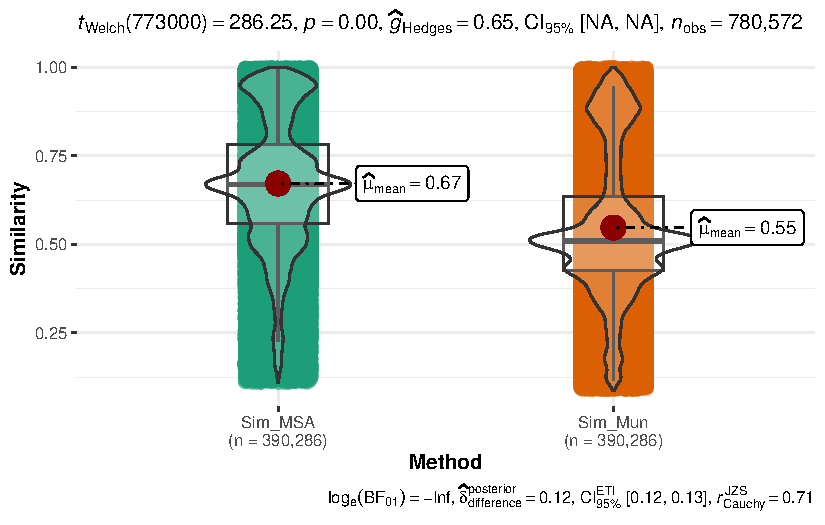
\includegraphics[width=0.3\textwidth,height=\textheight]{index_files/figure-pdf/unnamed-chunk-44-1.pdf}

}

\end{figure}

\begin{Shaded}
\begin{Highlighting}[]
\FunctionTok{boxplot}\NormalTok{(Sim\_comp[,}\FunctionTok{c}\NormalTok{(}\DecValTok{3}\NormalTok{,}\DecValTok{5}\NormalTok{)])}
\end{Highlighting}
\end{Shaded}

\begin{figure}[H]

{\centering 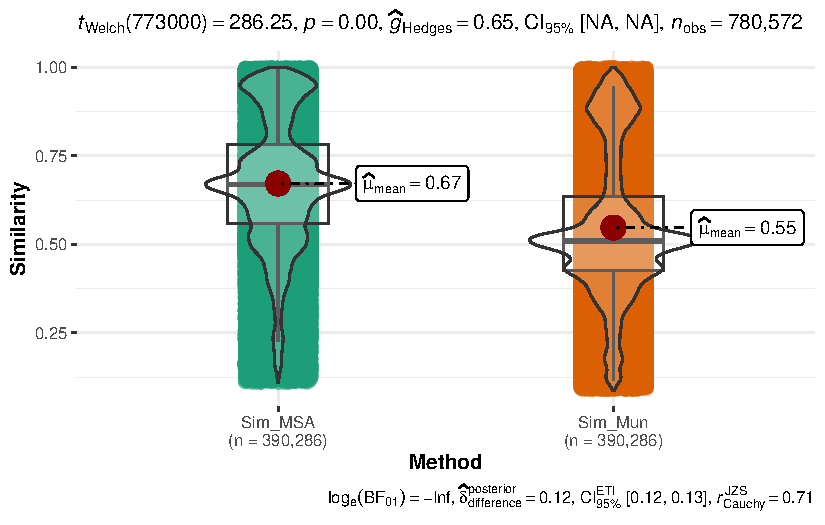
\includegraphics[width=0.3\textwidth,height=\textheight]{index_files/figure-pdf/unnamed-chunk-45-1.pdf}

}

\end{figure}

\bookmarksetup{startatroot}

\hypertarget{graph}{%
\chapter*{Graph}\label{graph}}
\addcontentsline{toc}{chapter}{Graph}

\markboth{Graph}{Graph}

Some statistics for graphs

\hypertarget{read-all-graphs-from-a-level-of-the-experiment}{%
\section*{Read all graphs from a level of the
experiment}\label{read-all-graphs-from-a-level-of-the-experiment}}
\addcontentsline{toc}{section}{Read all graphs from a level of the
experiment}

\markright{Read all graphs from a level of the experiment}

Read all graphs from a level from experiment; for example individuals.
We read only firts (alphabetic) two graph

\begin{Shaded}
\begin{Highlighting}[]
\NormalTok{path\_exp}\OtherTok{=}\StringTok{"data/results\_ff15c187{-}62e7{-}37c2{-}96a7{-}c824f7eab671/data/"}
\NormalTok{list\_names}\OtherTok{=}\FunctionTok{dir}\NormalTok{(}\FunctionTok{paste0}\NormalTok{(path\_exp,}\StringTok{"Individuals/"}\NormalTok{))}

\NormalTok{list\_names}\OtherTok{=}\NormalTok{ list\_names[}\SpecialCharTok{{-}}\DecValTok{1}\NormalTok{] }\CommentTok{\# filter 0000\_RefPw}
\FunctionTok{length}\NormalTok{(list\_names)}
\end{Highlighting}
\end{Shaded}

\begin{verbatim}
[1] 884
\end{verbatim}

\begin{Shaded}
\begin{Highlighting}[]
\NormalTok{graphs\_list}\OtherTok{=}\FunctionTok{paste0}\NormalTok{(path\_exp,}\StringTok{"Individuals/"}\NormalTok{,list\_names,}\StringTok{"/"}\NormalTok{,list\_names,}\StringTok{"\_MDAG.graphml"}\NormalTok{)}
\end{Highlighting}
\end{Shaded}

\begin{Shaded}
\begin{Highlighting}[]
\NormalTok{knitr}\SpecialCharTok{::}\FunctionTok{include\_graphics}\NormalTok{(}
  \FunctionTok{paste0}\NormalTok{(path\_exp,}\StringTok{"Individuals/cang/cang\_mDAG.pdf"}\NormalTok{))}
\end{Highlighting}
\end{Shaded}

\begin{figure}[H]

{\centering 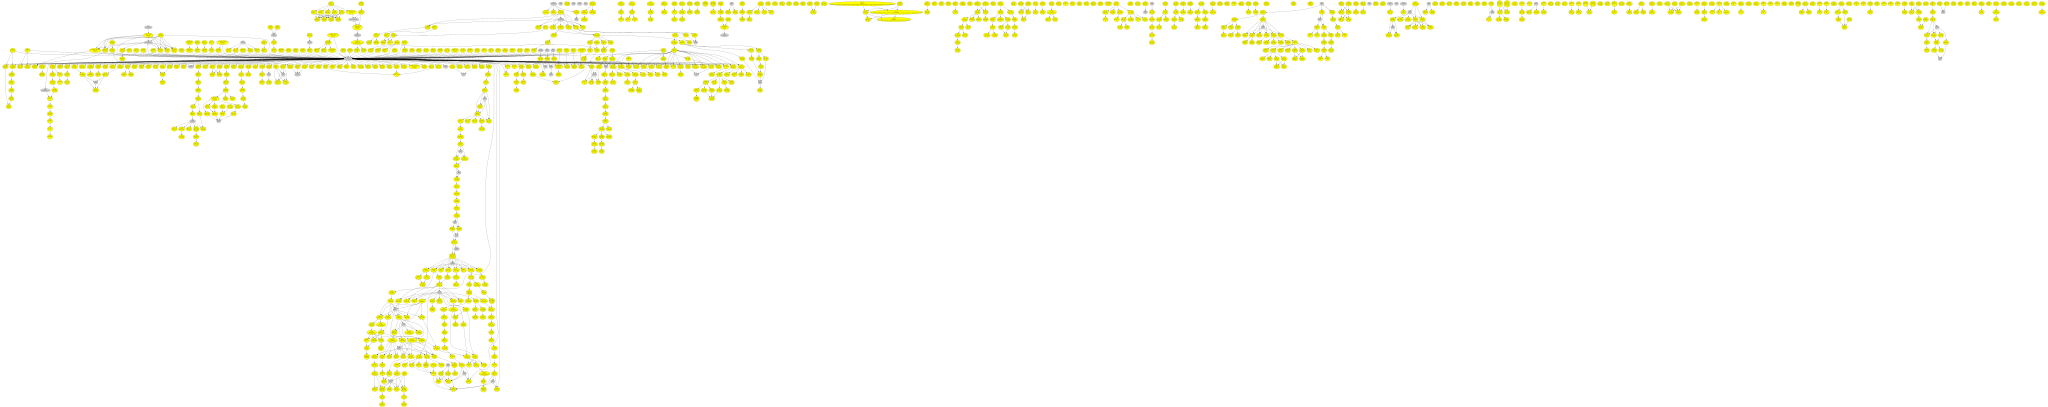
\includegraphics[width=0.3\textwidth,height=\textheight]{data/results_ff15c187-62e7-37c2-96a7-c824f7eab671/data/Individuals/cang/cang_mDAG.pdf}

}

\end{figure}

\begin{Shaded}
\begin{Highlighting}[]
\NormalTok{knitr}\SpecialCharTok{::}\FunctionTok{include\_graphics}\NormalTok{(}\FunctionTok{paste0}\NormalTok{(path\_exp,}\StringTok{"Individuals/cang/cang\_mDAG\_essential.pdf"}\NormalTok{))}
\end{Highlighting}
\end{Shaded}

\begin{figure}[H]

{\centering 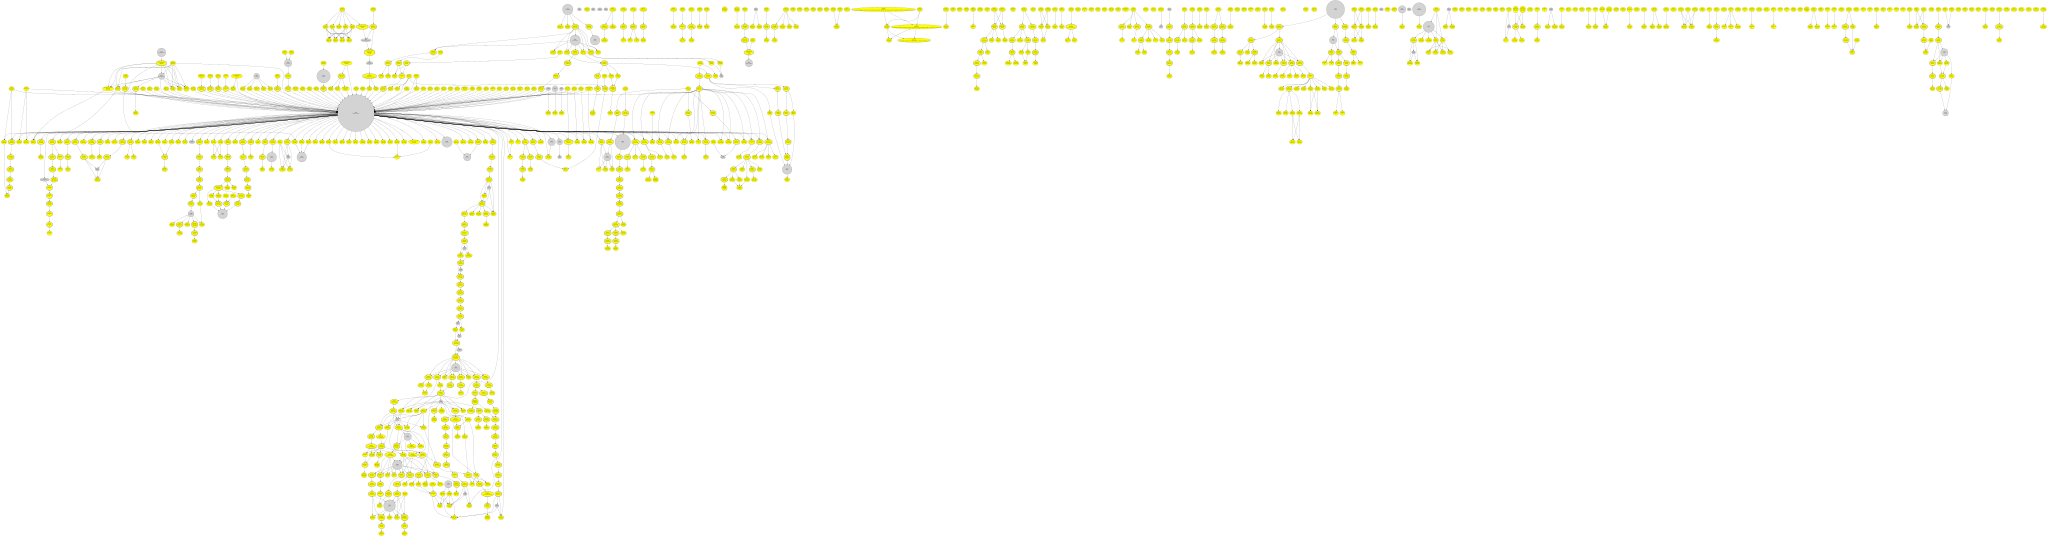
\includegraphics[width=0.3\textwidth,height=\textheight]{data/results_ff15c187-62e7-37c2-96a7-c824f7eab671/data/Individuals/cang/cang_mDAG_essential.pdf}

}

\end{figure}

\begin{Shaded}
\begin{Highlighting}[]
\NormalTok{knitr}\SpecialCharTok{::}\FunctionTok{include\_graphics}\NormalTok{(}
  \FunctionTok{paste0}\NormalTok{(path\_exp,}\StringTok{"Individuals/cang/cang\_RC.pdf"}\NormalTok{))}
\end{Highlighting}
\end{Shaded}

\begin{figure}[H]

{\centering \includegraphics[width=0.3\textwidth,height=\textheight]{data/results_ff15c187-62e7-37c2-96a7-c824f7eab671/data/Individuals/cang/cang_RC.pdf}

}

\end{figure}

\hypertarget{graph-statistics}{%
\section*{Graph statistics}\label{graph-statistics}}
\addcontentsline{toc}{section}{Graph statistics}

\markright{Graph statistics}

\begin{Shaded}
\begin{Highlighting}[]
\NormalTok{read\_mDAG}\OtherTok{=}\ControlFlowTok{function}\NormalTok{(x) \{DAG}\OtherTok{=}\FunctionTok{read.graph}\NormalTok{(}\AttributeTok{file=}\NormalTok{x,}
                                  \AttributeTok{format=}\StringTok{"graphml"}\NormalTok{)}
  \FunctionTok{return}\NormalTok{(DAG)\}}
\NormalTok{mDAG\_componets}\OtherTok{=}\ControlFlowTok{function}\NormalTok{(x) \{}\FunctionTok{sort}\NormalTok{(}\FunctionTok{components}\NormalTok{(x,}\AttributeTok{mode =} \StringTok{"weak"}\NormalTok{)}\SpecialCharTok{$}\NormalTok{csize,}
                                 \AttributeTok{decreasing=}\ConstantTok{TRUE}\NormalTok{)\}}



\NormalTok{compo\_list}\OtherTok{=}\FunctionTok{lapply}\NormalTok{(graphs\_list,}
                  \AttributeTok{FUN=}\ControlFlowTok{function}\NormalTok{(x) \{}
\NormalTok{                    gg}\OtherTok{=}\FunctionTok{read\_mDAG}\NormalTok{(x)}
\NormalTok{                  aux}\OtherTok{=}\FunctionTok{list}\NormalTok{(}
                    \AttributeTok{mDAG\_componets=}\FunctionTok{mDAG\_componets}\NormalTok{(gg),}
                    \AttributeTok{degree\_count=}\NormalTok{igraph}\SpecialCharTok{::}\FunctionTok{degree}\NormalTok{(gg,}\AttributeTok{mode=}\StringTok{"total"}\NormalTok{))}
                    \FunctionTok{return}\NormalTok{(aux)\}}
\NormalTok{                  )}

\FunctionTok{names}\NormalTok{(compo\_list)}\OtherTok{=}\NormalTok{list\_names}
\NormalTok{n}\OtherTok{=}\FunctionTok{max}\NormalTok{(}\FunctionTok{sapply}\NormalTok{(compo\_list,}\AttributeTok{FUN=}\ControlFlowTok{function}\NormalTok{(x) \{}\FunctionTok{length}\NormalTok{(x[[}\DecValTok{1}\NormalTok{]])\}))}
\NormalTok{n}
\end{Highlighting}
\end{Shaded}

\begin{verbatim}
[1] 234
\end{verbatim}

\begin{Shaded}
\begin{Highlighting}[]
\NormalTok{size\_compo\_list}\OtherTok{=}\FunctionTok{lapply}\NormalTok{(compo\_list,}\AttributeTok{FUN=}\ControlFlowTok{function}\NormalTok{(x) \{}
  \FunctionTok{return}\NormalTok{(}\FunctionTok{c}\NormalTok{(x[[}\DecValTok{1}\NormalTok{]],}\FunctionTok{rep}\NormalTok{(}\ConstantTok{NA}\NormalTok{,n}\SpecialCharTok{{-}}\FunctionTok{length}\NormalTok{(x[[}\DecValTok{1}\NormalTok{]]))))\})}

\NormalTok{aux}\OtherTok{=}\FunctionTok{do.call}\NormalTok{(bind\_cols,size\_compo\_list)}
\NormalTok{aux2}\OtherTok{=}\FunctionTok{pivot\_longer}\NormalTok{(aux,aaf}\SpecialCharTok{:}\NormalTok{zvi,}\AttributeTok{names\_to=}\StringTok{"Organism"}\NormalTok{,}
                  \AttributeTok{values\_to=}\StringTok{"csize"}\NormalTok{)}\SpecialCharTok{\%\textgreater{}\%}
  \FunctionTok{arrange}\NormalTok{(Organism,}\SpecialCharTok{{-}}\NormalTok{csize)}
\NormalTok{aux2}\SpecialCharTok{$}\NormalTok{index}\OtherTok{=}\FunctionTok{rep}\NormalTok{(}\DecValTok{1}\SpecialCharTok{:}\NormalTok{n,}\AttributeTok{times=}\FunctionTok{dim}\NormalTok{(aux)[}\DecValTok{2}\NormalTok{])}
\NormalTok{aux2}\OtherTok{=}\NormalTok{aux2 }\SpecialCharTok{\%\textgreater{}\%} \FunctionTok{left\_join}\NormalTok{(meta\_taxo,}\AttributeTok{by=}\StringTok{"Organism"}\NormalTok{)}
\end{Highlighting}
\end{Shaded}

\begin{Shaded}
\begin{Highlighting}[]
\NormalTok{Organism}\OtherTok{=}\FunctionTok{names}\NormalTok{(compo\_list)}
\NormalTok{big\_MBB}\OtherTok{=}\ControlFlowTok{function}\NormalTok{(org)\{}
\NormalTok{  x}\OtherTok{=}\NormalTok{Results }\SpecialCharTok{\%\textgreater{}\%} \FunctionTok{filter}\NormalTok{(Organism}\SpecialCharTok{==}\NormalTok{org)}
\NormalTok{  x}\OtherTok{=}\FunctionTok{as.character}\NormalTok{(x[}\DecValTok{1}\NormalTok{,}\DecValTok{5}\SpecialCharTok{:}\FunctionTok{dim}\NormalTok{(Results)[}\DecValTok{2}\NormalTok{]])}
\NormalTok{  x}\OtherTok{=}\NormalTok{x[x}\SpecialCharTok{!=}\StringTok{"NA"}\NormalTok{]}
\NormalTok{  tt}\OtherTok{=}\FunctionTok{sort}\NormalTok{(}\FunctionTok{table}\NormalTok{(x),}\AttributeTok{decreasing=}\ConstantTok{TRUE}\NormalTok{)}
  \FunctionTok{return}\NormalTok{(tt)}
\NormalTok{  \}}
\NormalTok{big\_MBB\_list}\OtherTok{=} \FunctionTok{lapply}\NormalTok{(Organism,}\AttributeTok{FUN=}\ControlFlowTok{function}\NormalTok{(x) }\FunctionTok{big\_MBB}\NormalTok{(x))}
\NormalTok{nMBB}\OtherTok{=}\FunctionTok{max}\NormalTok{(}\FunctionTok{sapply}\NormalTok{(big\_MBB\_list,}\AttributeTok{FUN=}\ControlFlowTok{function}\NormalTok{(x) }\FunctionTok{length}\NormalTok{(x)))}
\NormalTok{nMBB}
\end{Highlighting}
\end{Shaded}

\begin{verbatim}
[1] 1041
\end{verbatim}

\begin{Shaded}
\begin{Highlighting}[]
\NormalTok{big\_MBB\_list}\OtherTok{=}\FunctionTok{lapply}\NormalTok{(big\_MBB\_list,}
                    \AttributeTok{FUN=}\ControlFlowTok{function}\NormalTok{(x)\{}
\NormalTok{                      x}\OtherTok{=}\FunctionTok{c}\NormalTok{(x,}\FunctionTok{rep}\NormalTok{(}\ConstantTok{NA}\NormalTok{,nMBB}\SpecialCharTok{{-}}\FunctionTok{length}\NormalTok{(x)))}
                      \FunctionTok{return}\NormalTok{(x)\}}
\NormalTok{)}
\FunctionTok{names}\NormalTok{(big\_MBB\_list)}\OtherTok{=}\NormalTok{Organism}
\NormalTok{big\_MBB\_list}\OtherTok{=}\FunctionTok{do.call}\NormalTok{(bind\_cols,big\_MBB\_list)}

\NormalTok{kMBB}\OtherTok{=}\FunctionTok{nrow}\NormalTok{(big\_MBB\_list)}
\NormalTok{index}\OtherTok{=}\FunctionTok{rep}\NormalTok{(}\DecValTok{1}\SpecialCharTok{:}\NormalTok{kMBB,}\AttributeTok{times=}\FunctionTok{length}\NormalTok{(Organism))}

\NormalTok{big\_MBB\_list2}\OtherTok{=}\FunctionTok{pivot\_longer}\NormalTok{(big\_MBB\_list,}\AttributeTok{cols=}\FunctionTok{names}\NormalTok{(big\_MBB\_list),}\AttributeTok{values\_to =} \StringTok{"MBBsize"}\NormalTok{,}\AttributeTok{names\_to =} \StringTok{"Organism"}\NormalTok{) }\SpecialCharTok{\%\textgreater{}\%} \FunctionTok{arrange}\NormalTok{(Organism,}\SpecialCharTok{{-}}\NormalTok{MBBsize)}\SpecialCharTok{\%\textgreater{}\%}  \FunctionTok{mutate}\NormalTok{(}\AttributeTok{index=}\NormalTok{index) }\SpecialCharTok{\%\textgreater{}\%}  \FunctionTok{left\_join}\NormalTok{(meta\_taxo,}\AttributeTok{by=}\StringTok{"Organism"}\NormalTok{)}
\end{Highlighting}
\end{Shaded}

\hypertarget{sizes-of-mbb-for-each-mdag}{%
\subsection*{Sizes of MBB for each
mDAG}\label{sizes-of-mbb-for-each-mdag}}
\addcontentsline{toc}{subsection}{Sizes of MBB for each mDAG}

\begin{Shaded}
\begin{Highlighting}[]
\NormalTok{COLOR\_KINGDOM}\OtherTok{=}\FunctionTok{c}\NormalTok{(}\StringTok{"red"}\NormalTok{,}\StringTok{"black"}\NormalTok{,}\StringTok{"green"}\NormalTok{,}\StringTok{"yellow"}\NormalTok{)}
\NormalTok{colors\_kingdom}\OtherTok{=}\NormalTok{big\_MBB\_list2}\SpecialCharTok{\%\textgreater{}\%} \FunctionTok{select}\NormalTok{(Organism,Kingdom) }\SpecialCharTok{\%\textgreater{}\%} \FunctionTok{distinct}\NormalTok{()}
\FunctionTok{names}\NormalTok{(COLOR\_KINGDOM)}\OtherTok{=}\FunctionTok{sort}\NormalTok{(}\FunctionTok{unique}\NormalTok{(colors\_kingdom}\SpecialCharTok{$}\NormalTok{Kingdom))}

\NormalTok{p0}\OtherTok{\textless{}{-}}\FunctionTok{ggplot}\NormalTok{(}\AttributeTok{data=}\NormalTok{big\_MBB\_list2) }\SpecialCharTok{+} 
  \FunctionTok{geom\_line}\NormalTok{(}\AttributeTok{mapping=}\FunctionTok{aes}\NormalTok{(}\AttributeTok{x=}\NormalTok{index,}\AttributeTok{y=}\NormalTok{MBBsize,}\AttributeTok{group =}\NormalTok{ Organism,}\AttributeTok{color=}\NormalTok{Kingdom)) }\SpecialCharTok{+} 
  \FunctionTok{scale\_y\_continuous}\NormalTok{(}\AttributeTok{trans=}\StringTok{\textquotesingle{}log10\textquotesingle{}}\NormalTok{) }\SpecialCharTok{+} 
  \FunctionTok{scale\_x\_continuous}\NormalTok{(}\AttributeTok{trans=}\StringTok{\textquotesingle{}identity\textquotesingle{}}\NormalTok{) }\SpecialCharTok{+}
  \FunctionTok{scale\_color\_manual}\NormalTok{(}\AttributeTok{values =}\NormalTok{COLOR\_KINGDOM[colors\_kingdom}\SpecialCharTok{$}\NormalTok{Kingdom])}\SpecialCharTok{+}
   \FunctionTok{ggtitle}\NormalTok{(}\StringTok{"Plot log{-}identity of MBB }\SpecialCharTok{\textbackslash{}n}\StringTok{  decreasing index."}\NormalTok{) }\SpecialCharTok{+}
  \FunctionTok{ylab}\NormalTok{(}\StringTok{"Log10 MBB size"}\NormalTok{) }\SpecialCharTok{+} \FunctionTok{xlab}\NormalTok{(}\StringTok{"Index"}\NormalTok{)}


\NormalTok{p1}\OtherTok{\textless{}{-}} \FunctionTok{ggplot}\NormalTok{(}\AttributeTok{data=}\NormalTok{big\_MBB\_list2) }\SpecialCharTok{+} 
  \FunctionTok{geom\_line}\NormalTok{(}\AttributeTok{mapping=}\FunctionTok{aes}\NormalTok{(}\AttributeTok{x=}\NormalTok{index,}\AttributeTok{y=}\NormalTok{MBBsize,}\AttributeTok{group =}\NormalTok{ Organism,}\AttributeTok{color=}\NormalTok{Kingdom),}\AttributeTok{na.rm=}\ConstantTok{TRUE}\NormalTok{) }\SpecialCharTok{+} 
  \FunctionTok{scale\_x\_continuous}\NormalTok{(}\AttributeTok{trans=}\StringTok{\textquotesingle{}log10\textquotesingle{}}\NormalTok{) }\SpecialCharTok{+} 
  \FunctionTok{scale\_y\_continuous}\NormalTok{(}\AttributeTok{trans=}\StringTok{\textquotesingle{}log10\textquotesingle{}}\NormalTok{) }\SpecialCharTok{+}
  \FunctionTok{scale\_color\_manual}\NormalTok{(}\AttributeTok{values =}\NormalTok{COLOR\_KINGDOM[colors\_kingdom}\SpecialCharTok{$}\NormalTok{Kingdom])}\SpecialCharTok{+}
   \FunctionTok{ggtitle}\NormalTok{(}\StringTok{"Plot log10{-}log10identity of MBB }\SpecialCharTok{\textbackslash{}n}\StringTok{  decreasing index."}\NormalTok{) }\SpecialCharTok{+}
  \FunctionTok{ylab}\NormalTok{(}\StringTok{"Log10 MBB size"}\NormalTok{) }\SpecialCharTok{+} \FunctionTok{xlab}\NormalTok{(}\StringTok{"Log10 Index"}\NormalTok{)}

\NormalTok{p2}\OtherTok{\textless{}{-}} \FunctionTok{ggplot}\NormalTok{(}\AttributeTok{data=}\NormalTok{big\_MBB\_list2) }\SpecialCharTok{+} 
  \FunctionTok{geom\_line}\NormalTok{(}\AttributeTok{mapping=}\FunctionTok{aes}\NormalTok{(}\AttributeTok{x=}\NormalTok{index,}\AttributeTok{y=}\NormalTok{MBBsize,}\AttributeTok{group =}\NormalTok{ Organism,}\AttributeTok{color=}\NormalTok{Kingdom),}\AttributeTok{na.rm=}\ConstantTok{TRUE}\NormalTok{)}\SpecialCharTok{+}
   \FunctionTok{scale\_x\_continuous}\NormalTok{(}\AttributeTok{trans=}\StringTok{"identity"}\NormalTok{) }\SpecialCharTok{+} 
   \FunctionTok{scale\_y\_continuous}\NormalTok{(}\AttributeTok{trans=}\StringTok{"identity"}\NormalTok{) }\SpecialCharTok{+}
  \FunctionTok{ylim}\NormalTok{(}\DecValTok{0}\NormalTok{,}\DecValTok{1039}\NormalTok{)}\SpecialCharTok{+}
   \FunctionTok{ggtitle}\NormalTok{(}\StringTok{"Plot  of MBB sized  decreasing index."}\NormalTok{) }\SpecialCharTok{+}
  \FunctionTok{ylab}\NormalTok{(}\StringTok{"MBB size"}\NormalTok{) }\SpecialCharTok{+} \FunctionTok{xlab}\NormalTok{(}\StringTok{"Index"}\NormalTok{)}\SpecialCharTok{+}
  \FunctionTok{scale\_color\_manual}\NormalTok{(}\AttributeTok{values =}\NormalTok{COLOR\_KINGDOM[colors\_kingdom}\SpecialCharTok{$}\NormalTok{Kingdom])}

\FunctionTok{library}\NormalTok{(patchwork)}

\NormalTok{p0}
\end{Highlighting}
\end{Shaded}

\begin{figure}[H]

{\centering 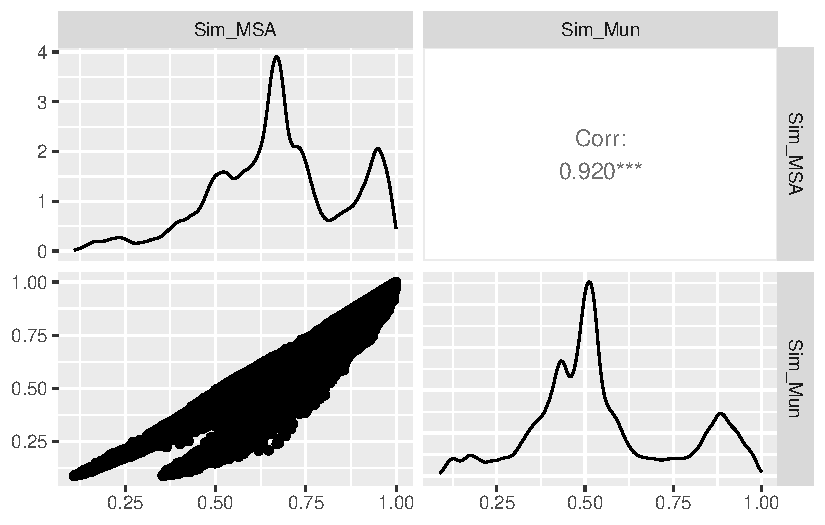
\includegraphics[width=0.3\textwidth,height=\textheight]{index_files/figure-pdf/unnamed-chunk-52-1.pdf}

}

\end{figure}

\begin{Shaded}
\begin{Highlighting}[]
\NormalTok{p1}
\end{Highlighting}
\end{Shaded}

\begin{figure}[H]

{\centering \includegraphics[width=0.3\textwidth,height=\textheight]{index_files/figure-pdf/unnamed-chunk-52-2.pdf}

}

\end{figure}

\begin{Shaded}
\begin{Highlighting}[]
\NormalTok{p2}
\end{Highlighting}
\end{Shaded}

\begin{figure}[H]

{\centering \includegraphics[width=0.3\textwidth,height=\textheight]{index_files/figure-pdf/unnamed-chunk-52-3.pdf}

}

\end{figure}

\hypertarget{sizes-of-weak-components-for-each-mdag}{%
\subsection*{Sizes of weak components for each
mDAG}\label{sizes-of-weak-components-for-each-mdag}}
\addcontentsline{toc}{subsection}{Sizes of weak components for each
mDAG}

\begin{Shaded}
\begin{Highlighting}[]
\NormalTok{COLOR\_KINGDOM}\OtherTok{=}\FunctionTok{c}\NormalTok{(}\StringTok{"red"}\NormalTok{,}\StringTok{"black"}\NormalTok{,}\StringTok{"green"}\NormalTok{,}\StringTok{"yellow"}\NormalTok{)}
\NormalTok{colors\_kingdom}\OtherTok{=}\NormalTok{aux2}\SpecialCharTok{\%\textgreater{}\%} \FunctionTok{select}\NormalTok{(Organism,Kingdom) }\SpecialCharTok{\%\textgreater{}\%} \FunctionTok{distinct}\NormalTok{()}
\FunctionTok{names}\NormalTok{(COLOR\_KINGDOM)}\OtherTok{=}\FunctionTok{sort}\NormalTok{(}\FunctionTok{unique}\NormalTok{(colors\_kingdom}\SpecialCharTok{$}\NormalTok{Kingdom))}

\NormalTok{p0}\OtherTok{\textless{}{-}}\FunctionTok{ggplot}\NormalTok{(}\AttributeTok{data=}\NormalTok{aux2) }\SpecialCharTok{+} 
  \FunctionTok{geom\_line}\NormalTok{(}\AttributeTok{mapping=}\FunctionTok{aes}\NormalTok{(}\AttributeTok{x=}\NormalTok{index,}\AttributeTok{y=}\NormalTok{csize,}\AttributeTok{group =}\NormalTok{ Organism,}\AttributeTok{color=}\NormalTok{Kingdom),}\AttributeTok{na.rm=}\ConstantTok{TRUE}\NormalTok{) }\SpecialCharTok{+} 
  \FunctionTok{scale\_x\_continuous}\NormalTok{(}\AttributeTok{trans=}\StringTok{\textquotesingle{}log10\textquotesingle{}}\NormalTok{) }\SpecialCharTok{+} 
  \FunctionTok{scale\_y\_continuous}\NormalTok{(}\AttributeTok{trans=}\StringTok{\textquotesingle{}identity\textquotesingle{}}\NormalTok{) }\SpecialCharTok{+}
  \FunctionTok{scale\_color\_manual}\NormalTok{(}\AttributeTok{values =}\NormalTok{COLOR\_KINGDOM[colors\_kingdom}\SpecialCharTok{$}\NormalTok{Kingdom])}\SpecialCharTok{+}
   \FunctionTok{ggtitle}\NormalTok{(}\StringTok{"Plot log{-}identity of size  weak components decreasing index."}\NormalTok{) }\SpecialCharTok{+}
  \FunctionTok{ylab}\NormalTok{(}\StringTok{"Log10 Weak componente size"}\NormalTok{) }\SpecialCharTok{+} \FunctionTok{xlab}\NormalTok{(}\StringTok{"Index"}\NormalTok{)}


\NormalTok{p1}\OtherTok{\textless{}{-}} \FunctionTok{ggplot}\NormalTok{(}\AttributeTok{data=}\NormalTok{aux2) }\SpecialCharTok{+} 
  \FunctionTok{geom\_line}\NormalTok{(}\AttributeTok{mapping=}\FunctionTok{aes}\NormalTok{(}\AttributeTok{x=}\NormalTok{index,}\AttributeTok{y=}\NormalTok{csize,}\AttributeTok{group =}\NormalTok{ Organism,}\AttributeTok{color=}\NormalTok{Kingdom),}\AttributeTok{na.rm=}\ConstantTok{TRUE}\NormalTok{) }\SpecialCharTok{+} 
  \FunctionTok{scale\_y\_continuous}\NormalTok{(}\AttributeTok{trans=}\StringTok{\textquotesingle{}log10\textquotesingle{}}\NormalTok{) }\SpecialCharTok{+} 
  \FunctionTok{scale\_x\_continuous}\NormalTok{(}\AttributeTok{trans=}\StringTok{\textquotesingle{}log10\textquotesingle{}}\NormalTok{) }\SpecialCharTok{+}
  \FunctionTok{scale\_color\_manual}\NormalTok{(}\AttributeTok{values =}\NormalTok{COLOR\_KINGDOM[colors\_kingdom}\SpecialCharTok{$}\NormalTok{Kingdom])}\SpecialCharTok{+}
   \FunctionTok{ggtitle}\NormalTok{(}\StringTok{"Plot log{-}log of size  weak components decreasing index."}\NormalTok{) }\SpecialCharTok{+}
  \FunctionTok{ylab}\NormalTok{(}\StringTok{"Log10 weak component size"}\NormalTok{) }\SpecialCharTok{+} \FunctionTok{xlab}\NormalTok{(}\StringTok{"Log10 Index"}\NormalTok{)}

\NormalTok{p2}\OtherTok{\textless{}{-}} \FunctionTok{ggplot}\NormalTok{(}\AttributeTok{data=}\NormalTok{aux2) }\SpecialCharTok{+} 
  \FunctionTok{geom\_line}\NormalTok{(}\AttributeTok{mapping=}\FunctionTok{aes}\NormalTok{(}\AttributeTok{x=}\NormalTok{index,}\AttributeTok{y=}\NormalTok{csize,}\AttributeTok{group =}\NormalTok{ Organism,}\AttributeTok{color=}\NormalTok{Kingdom),}\AttributeTok{na.rm=}\ConstantTok{TRUE}\NormalTok{) }\SpecialCharTok{+} 
   \FunctionTok{scale\_x\_continuous}\NormalTok{(}\AttributeTok{trans=}\StringTok{"identity"}\NormalTok{) }\SpecialCharTok{+} 
  \FunctionTok{scale\_y\_continuous}\NormalTok{(}\AttributeTok{trans=}\StringTok{"identity"}\NormalTok{) }\SpecialCharTok{+}
  \FunctionTok{ylim}\NormalTok{(}\DecValTok{0}\NormalTok{,}\DecValTok{1039}\NormalTok{)}\SpecialCharTok{+}
   \FunctionTok{ggtitle}\NormalTok{(}\StringTok{"Plot  of size  weak components decreasing index."}\NormalTok{)}\SpecialCharTok{+}  \FunctionTok{ylab}\NormalTok{(}\StringTok{"Weak components size"}\NormalTok{) }\SpecialCharTok{+} \FunctionTok{xlab}\NormalTok{(}\StringTok{"Index"}\NormalTok{)}\SpecialCharTok{+}
  \FunctionTok{scale\_color\_manual}\NormalTok{(}\AttributeTok{values =}\NormalTok{COLOR\_KINGDOM[colors\_kingdom}\SpecialCharTok{$}\NormalTok{Kingdom])}

\FunctionTok{library}\NormalTok{(patchwork)}

\NormalTok{p0}
\end{Highlighting}
\end{Shaded}

\begin{figure}[H]

{\centering 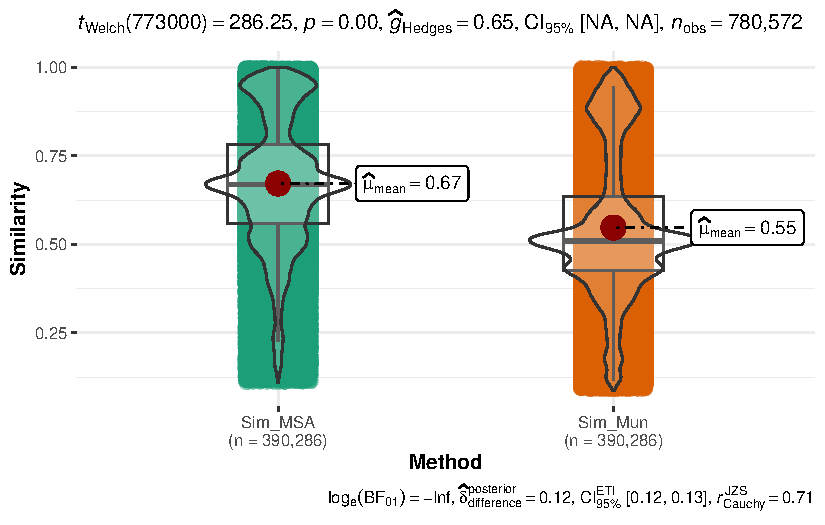
\includegraphics[width=0.3\textwidth,height=\textheight]{index_files/figure-pdf/unnamed-chunk-53-1.pdf}

}

\end{figure}

\begin{Shaded}
\begin{Highlighting}[]
\NormalTok{p1}
\end{Highlighting}
\end{Shaded}

\begin{figure}[H]

{\centering \includegraphics[width=0.3\textwidth,height=\textheight]{index_files/figure-pdf/unnamed-chunk-53-2.pdf}

}

\end{figure}

\begin{Shaded}
\begin{Highlighting}[]
\NormalTok{p2}
\end{Highlighting}
\end{Shaded}

\begin{figure}[H]

{\centering \includegraphics[width=0.3\textwidth,height=\textheight]{index_files/figure-pdf/unnamed-chunk-53-3.pdf}

}

\end{figure}

\begin{Shaded}
\begin{Highlighting}[]
\NormalTok{data2}\OtherTok{=}\NormalTok{big\_MBB\_list2 }\SpecialCharTok{\%\textgreater{}\%} \FunctionTok{filter}\NormalTok{(index}\SpecialCharTok{!=}\DecValTok{1}\NormalTok{)}
\NormalTok{p3}\OtherTok{\textless{}{-}} \FunctionTok{ggplot}\NormalTok{(}\AttributeTok{data=}\NormalTok{data2) }\SpecialCharTok{+} 
  \FunctionTok{geom\_line}\NormalTok{(}\AttributeTok{mapping=}\FunctionTok{aes}\NormalTok{(}\AttributeTok{x=}\NormalTok{index,}\AttributeTok{y=}\NormalTok{MBBsize,}\AttributeTok{group =}\NormalTok{ Organism,}\AttributeTok{color=}\NormalTok{Kingdom),}\AttributeTok{na.rm=}\ConstantTok{TRUE}\NormalTok{)}\SpecialCharTok{+}
   \FunctionTok{scale\_x\_continuous}\NormalTok{(}\AttributeTok{trans=}\StringTok{"identity"}\NormalTok{) }\SpecialCharTok{+} 
  \FunctionTok{scale\_y\_continuous}\NormalTok{(}\AttributeTok{trans=}\StringTok{"identity"}\NormalTok{) }\SpecialCharTok{+}
  \FunctionTok{ylim}\NormalTok{(}\DecValTok{0}\NormalTok{,}\DecValTok{25}\NormalTok{)}\SpecialCharTok{+}
   \FunctionTok{ggtitle}\NormalTok{(}\StringTok{"Plot  of size  weak components decreasing index."}\NormalTok{)}\SpecialCharTok{+}  \FunctionTok{ylab}\NormalTok{(}\StringTok{"Weak components size"}\NormalTok{) }\SpecialCharTok{+} \FunctionTok{xlab}\NormalTok{(}\StringTok{"Index"}\NormalTok{)}\SpecialCharTok{+}
  \FunctionTok{scale\_color\_manual}\NormalTok{(}\AttributeTok{values =}\NormalTok{COLOR\_KINGDOM[colors\_kingdom}\SpecialCharTok{$}\NormalTok{Kingdom])}

\NormalTok{p3}
\end{Highlighting}
\end{Shaded}

\begin{figure}[H]

{\centering \includegraphics[width=0.3\textwidth,height=\textheight]{index_files/figure-pdf/unnamed-chunk-54-1.pdf}

}

\end{figure}



\end{document}
